%%%%%%%%%%%%%%%%%%%%%%%%%%%%%%%%%%%%%%%%%%%%%%%%%%%%%%%%%%%%%%%%%%%%%%%%%%%%%%%
%%%%%%%%%%%%%%%%%%%%%%%%%%%%%%%%%%%%%%%%%%%%%%%%%%%%%%%%%%%%%%%%%%%%%%%%%%%%%%%
%%%%  CHAPTER 9
%%%%%%%%%%%%%%%%%%%%%%%%%%%%%%%%%%%%%%%%%%%%%%%%%%%%%%%%%%%%%%%%%%%%%%%%%%%%%%%
%%%%%%%%%%%%%%%%%%%%%%%%%%%%%%%%%%%%%%%%%%%%%%%%%%%%%%%%%%%%%%%%%%%%%%%%%%%%%%%
\chapter{Diagnostic tools IV:  Bragg scattering of light}
\label{chap:bragg-scatt}

The most important contribution of our work has been the development of Bragg
scattering thermometry for ultracold atoms in optical lattices.  This kind of
thermometry exploits the long range spin order that develops in the system
below the N\'{e}el transition temperature, $T_{N}$.   The idea behind Bragg
scattering is very simple:  a wave scattered coherently from a periodic
ensemble of particles will show enhanced scattering at certain directions,
depending on the angle of the incoming light and the periodic pattern of the
ensemble.  In the case of ultracold atoms the wave used is
light~\cite{PhysRevLett.75.2823,Weidemueller1998}, with frequency close to an
atomic resonance in order to have a significant cross section.  In materials
science and crystallography,  Bragg scattering of X-rays and neutrons is
routinely used to characterize samples.   The internal structure of the
scatterers, in addition to their periodic arrangement,  also affects the
angular distribution of the scattered light.  As a notable example,  X-ray
scattering was used to infer the double-helix structure of DNA.  In the case of
ultracold atoms, Bragg scattering can be used to measure the spatial extent and
coherence of atomic wavefunctions~\cite{Miyake2011}, and also the spin ordering
of the ensemble of atoms~\cite{Hart2014arxiv}.

It is clear that below $T_{N}$, long range spin ordering will give rise to a
large Bragg signal, proportional to the square of the number of atoms in a
hypothetical AFM domain.   Above $T_{N}$, antiferromagnetic (AFM) correlations
start to develop as the  system approaches the transition.   It was unclear
whether it would be possible to experimentally detect  the weak AFM
correlations, however, in the end we find the signal to be detectable if one
has enough statistics from repeating the experiment many times.

Modeling the Bragg scattering experiment with ultracold atoms is very simple if
one considers the far-detuned or weak intensity limit,  where all of the light
is scattered coherently by the atoms. In this regime the electric field
scattered by each of the atoms is exactly in phase with the electric field of
the incident light, and inelastic light scattering (which results in a field
with a random phase) can be neglected.  Demonstrations of Bragg scattering with
ultracold atoms typically operate in this
regime~\cite{PhysRevLett.75.2823,PhysRevLett.75.4583,Miyake2011}.  There has
also been theoretical work which suggests ways to exploit the  characteristics
of the scattered light to probe the many body states that form in an optical
lattice~\cite{Ted2010, PhysRevX.4.031036};  however, those results are also in
the context of a very weak probe and do not consider the effects of saturation
of the atomic transition.  

When performing Bragg scattering to detect the spin ordering of atoms in a
lattice, one must have a spin-sensitive probe, i.e.  light that scatters
differently from atoms in states $|1\rangle$ and $|2\rangle$.   The phase shift
$\delta$ of the scattered light is related to the detuning $\Delta$ (in units
of the linewidth)  from the atomic transition as $\tan{\delta} \propto
\Delta^{-1}$.  If one sets the light detuning right in between the two states,
then $\Delta_{\spup} = -\Delta_{\spdn}$, and light scattered from one state
will have a $\pi$ phase shift with respect to light scattered from the other
one\footnote{Note that $\tan[\delta+\pi]=-\tan\delta$.}, as shown in
Fig.~\ref{fig:spin-sense}.    
\begin{figure}
    \centering
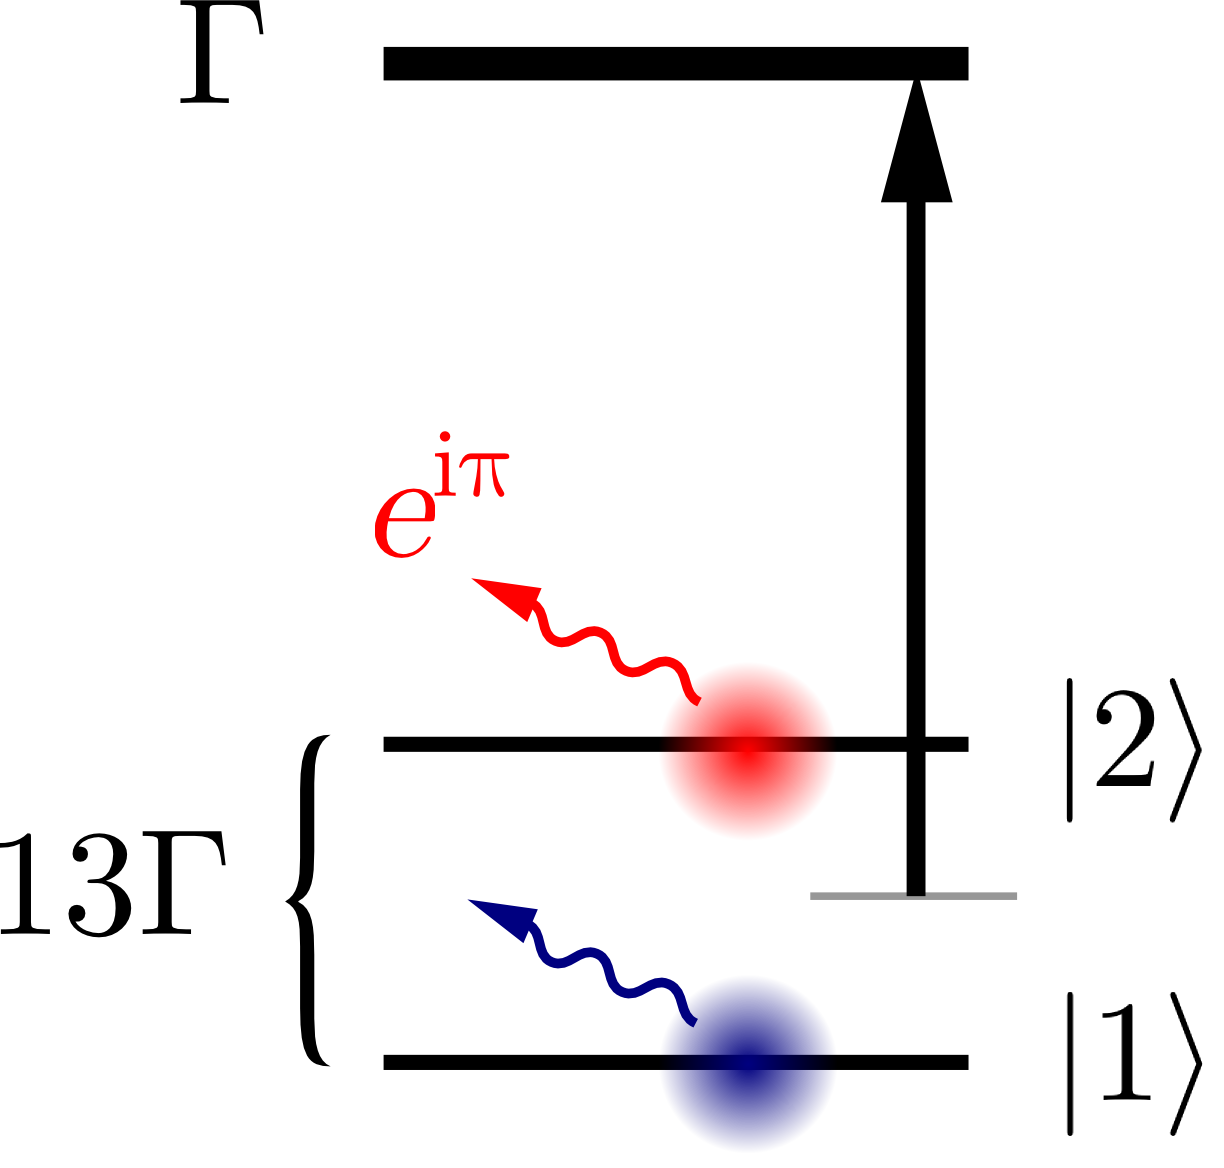
\includegraphics[width=0.3\textwidth]{../figures/braggscatt/spin-sensitive12.png}
\caption{\small Illustration of spin-sensitive light scattering. }
\label{fig:spin-sense}
\end{figure} 
We find experimentally that, to obtain a measurable scattering signal, we must
use probe parameters that are not in the far-detuned or weak intensity ideal
scenarios.  The detuning is fixed by the requirement to have a spin-sensitive
measurement,  the power of the probe is determined by the signal to noise ratio
of our detection setup,  and the duration is constrained by the effects on the
center of mass state of the atoms due to the recoil from every photon
scattered. 
 

This chapter starts out with a detailed derivation of the equations for light
scattering by an array of atoms, including saturation effects of the transition
via the optical Bloch equations.   We will then introduce the experimental
setup that was constructed for Bragg scattering.   Finally we will show results
for a measurement of the crystalline structure of the optical lattice using
Bragg scattering.  These results will serve as an illustration of the power of
this technique.   Details of the measurement of AFM correlations using
spin-sensitive light scattering will be deferred until
Chapter~\ref{chap:afmbragg}.  
 
\section{Coherent light scattering by an array of atoms. } 

For a collection of two-level atoms, the steady-state scattered intensity
measured at a detector can be obtained by coherently adding up the field
emitted by all the atoms and squaring it to find the intensity.

%The spin
%structure factor is defined (Eq.~1) as a sum over lattice sites $i,\,j$:
%\begin{equation}
%    S_{\bv{Q}} = \frac{4}{N} \sum_{i,j}
%     e^{i\bv{Q}\cdot ( \bv{R}_{i} - \bv{R}_{j} )}
%      \langle \sigma_{zi} \sigma_{zj}  \rangle
%\end{equation}
%By quickly ramping the lattice depth to $v_{0}=20E_{r}$, the state of the
%system is projected into a product state, where the wavefunction of each atom
%is localised at a lattice site. Hence, we can write $S_{\bv{Q}}$ as a sum over
%particles $m,n$:
%\begin{equation}
%    S_{\bv{Q}} = \frac{4}{N} \sum_{m,n}
%     e^{i\bv{Q}\cdot ( \bv{R}_{m} - \bv{R}_{n} )}
%      \langle \sigma_{z} \rangle_{m} \langle \sigma_{z}  \rangle_{n}
%\label{eq:sqdef}
%\end{equation}
%where $\langle \sigma_{z} \rangle_{n}$ is the $z$ component of the spin of the
%$n^{\text{th}}$ atom.


When illuminated with probe light with wavevector $\bv{k}$ (magnitude
$k=|\bv{k}|$) and angular frequency $\omega_{\text{p}}$, the $n^{\text{th}}$
atom emits a field proportional to its dipole
moment~\cite{cohen1998atom,Ruostekoski2009}:
\begin{equation}
  \bv{E}_{n}^{+}  =
  \frac{ 1 }{ \sqrt{ 2 \epsilon_{0} c }}
    \left[ \frac{3}{8\pi} \frac{ \hbar c k \Gamma }{ r_{D}^{2}} \right]^{1/2}
   \bv{\Lambda} \,\,
    e^{i(\bv{k}'-\bv{k} ) \cdot \hat{\bv{r}}_{n} }
   \varsigma_{n-}
 \label{eq:epropsigma}
\end{equation}
where
\begin{itemize}

\item $\bv{E}_{n}^{+}$ is the positive frequency component of the electric
field amplitude at a point in space that is a distance $r_{D}$ from the sample
in the direction of the wavevector of the scattered light 

\item $c$ is the speed of light, $\epsilon_{0}$ is the vacuum permittivity,
$\hbar$ is Planck's constant divided by $2\pi$. 

\item  $\Gamma$ is the linewidth of the transition

\item $\bv{k}'$ is the wave vector of the scattered light 

\item $\hat{\bv{r}}_{n}$ is the position operator of the $n^{\text{th}}$ atom

\item $\bv{\Lambda} = \bv{k}' \times ( \bv{k}' \times \bv{\mathrm{d}}_{ge})/ (
k'^{2}| \bv{\mathrm{d}}_{ge}|)$ is the polarization vector of the field (dipole
radiation pattern)
 
\item 
%where $\hat{\bv{n}} = \bv{k'}/|\bv{k'}|$, 
$\bv{\mathrm{d}}_{ge} = \langle g | \bv{\mathrm{d}} | e \rangle$  is the
transition matrix element between the ground $|g\rangle$ and excited
$|e\rangle$ electronic states

\item $\varsigma_{n-} = e^{i\omega_{\text{p}}t} |g\rangle\langle e|$ is the
off-diagonal matrix element of the atomic density matrix in the rotating frame
\end{itemize}

The two atomic states, $|\nSspup\rangle$ and $|\nSspdn\rangle$, only differ in
the projection of the nuclear spin,  so $\bv{\mathrm{d}}_{ge}$ is the same for
either state.  For this reason, we make no distinction of the spin part of the
wavefunction in states  $|e\rangle$ and $|g\rangle$.  Both states
$|\nSspup\rangle$, $|\nSspdn\rangle$ have an electronic angular momentum
projection $m_{J}=-1/2$ and the respective excited states have $m_{J}=-3/2$.
The matrix element can then be written as $\bv{\mathrm{d}}_{ge}
=|\bv{\mathrm{d}}_{ge}| \hat{\bv{e}}_{-1} $  (as for any
$\Delta m_{J}=-1$ transition).

The intensity at the detector, for a momentum transfer $\bv{Q}=\bv{k}'-\bv{k}$,
can be obtained by summing the field contributions from the individual atoms
and squaring the total field:
\begin{equation}
 I_{\bv{Q}}  =
  2 \epsilon_{0} c \
    \langle \Psi \big|  \left(  \sum_{m}  \bv{E}_{m}^{-} \right) \cdot
           \left(  \sum_{n} \bv{E}_{n}^{+} \right) \big|  \Psi\rangle.
  \label{eq:isum}
\end{equation}
Here $|\Psi\rangle$ is the product state of the array of atoms:  $|\Psi\rangle
= \prod_{n} |u \rangle_{n} |\sigma \rangle_{n}$ where $u$ and $\sigma$
represent the center of mass and electronic states of the atom respectively.
The wavefunction for the system of atoms in the lattice (which in general can
be a highly entangled many-body state) must be projected into a product state
(like $|\Psi\rangle$)  before performing the measurement.  This is achieved by
quickly ramping the lattice depth up to $20\,E_{r}$,  which projects the state
of the system into a state with a well defined atom number in each site, and
prevents further tunneling during the measurement.  

The projection to a product state helps simplify the interpretation of the
scattered intensity measurements.  The projected state in a deep lattice will
allow us to neglect changes of the center of mass state of the system during
scattering.  Calculating the properties of the scattered light starting from
the full many-body wavefunction, rather than a projected state can reveal more
of the properties of the many-body state, but it is a difficult
task~\cite{PhysRevX.4.031036}.

Using Eq.~\ref{eq:epropsigma} inside Eq.~\ref{eq:isum} and separating the sum
into off-diagonal and diagonal terms yields
\begin{equation}
\begin{split}
 I_{\bv{Q}} = &
  A\left[
    \sumOff \langle \varsigma_{n+}\rangle \langle \varsigma_{m-} \rangle
\langle u | e^{-i(\bv{k}'-\bv{k} ) \cdot \hat{\bv{r}}_{m} } | u \rangle_{m} 
 \langle u | 
e^{i(\bv{k}'-\bv{k} ) \cdot \hat{\bv{r}}_{n} }| u \rangle_{n}  \right.
  \left.  + \sum_{n}  \langle \varsigma_{n+} \varsigma_{n-} \rangle
\right]
\end{split}
\label{eq:IQsum}
\end{equation}
where $A = \frac{3}{8\pi} \frac{\hbar c k
\Gamma}{r_{D}^{2}}|\bv{\Lambda}|^{2}$.   


We assume that the center of mass state for all atoms is the harmonic
oscillator ground state of a single site
\begin{equation} 
   |u\rangle_{m}  = |0\rangle_{m}
\end{equation}
We also neglect the possibility of an atom recoiling to a different center of
mass state. The center of mass expectation value that appears inside the sum in
Eq.~\ref{eq:IQsum} is evaluated by first performing a translation $\bv{R}_{m}$
of the coordinate system for each term, such that the position of the
$m^{\text{th}}$ atom has a zero expectation value $\langle \bv{r}_{m}
\rangle=0$,  and then using the identity $\langle e^{\hat{A}} \rangle =
e^{\frac{1}{2} \langle \hat{A}^{2} \rangle}$, which is valid for a simple
harmonic oscillator eigenstate if $\hat{A}$ is a linear combination of
displacement and momentum operators of the oscillator.  
\begin{equation}
\begin{split}
      \langle u | e^{-i(\bv{k}'-\bv{k}) \cdot\hat{\bv{r}}_{m}} | u  \rangle_{m} = & 
      \langle 0 | e^{-i(\bv{k}'-\bv{k}) \cdot\hat{\bv{r}}_{m}} | 0  \rangle_{m} \\
    = & e^{-i(\bv{k}'-\bv{k}) \cdot\bv{R}_{m}} 
      e^{ -\frac{1}{2} \left\langle 
          [ (\bv{k}'-\bv{k}) \cdot\hat{\bv{r}}_{m} ]^{2} \right\rangle } \\
    = & e^{ -i \bv{Q} \cdot \bv{R}_{m}} 
      e^{ -\frac{1}{2} \left\langle [ \bv{Q} \cdot\hat{\bv{r}}_{m} ]^{2} \right\rangle } \\ 
    = & e^{ -i \bv{Q} \cdot \bv{R}_{m}}
      \prod_{i=x,y,z} e^{ - \frac{1}{2}Q_{i}^{2}\langle r_{mi} ^{2} \rangle } \\ 
    = & e^{ -i \bv{Q} \cdot \bv{R}_{m}}
      e^{-W_{\bv{Q}}(\tau)} 
\end{split}
\end{equation} 
Plugging the center of mass expectation value back into Eq.~\ref{eq:IQsum} we
obtain 
\begin{equation}
 I_{\bv{Q}} / A     =
  \debyew
    \sumOff \langle \varsigma_{n+}\rangle \langle \varsigma_{m-} \rangle
  e^{ i \bv{Q} \cdot ( \bv{R}_{n} - \bv{R}_{m} ) }
   + \sum_{n}  \langle \varsigma_{n+} \varsigma_{n-} \rangle.
 \label{eq:IQresult}
\end{equation}
Here \debyew\ is the Debye-Waller factor defined as
\begin{equation}
  \debyew  = \prod_{i=x,y,z} e^{-Q_{i}^{2} 
              \langle \hat{r}_{i}^{2} \rangle_{\tau} }
\label{eq:define-debyew}
\end{equation}
where $\langle r_{i}^{2} \rangle_{\tau}$ is the variance in the $i^{\text{th}}$
coordinate of an atom, assumed to be the same for all atoms in the array.   The
variance depends on the time-of-flight $\tau$;  as we will see, for some
measurements the atoms are released in time-of-flight before probing them with
the light. 

The resulting intensity in Eq.~\ref{eq:IQresult} is seen to be the result of
two contributions.  The first one is a result of the interference of the field
scattered by all the atoms in the ensemble.  The magnitude of this contribution
is multiplied by the Debye-Waller factor,  which is related to the spatial
extent of an atomic wavefunction.   	The second part, which is proportional
to the number of atoms, corresponds to the non-interfering part of the
scattered light;  what we would obtain if we were to add up the intensities of
scattering by individual atoms. 

The steady-state solutions to the optical Bloch equations can be used to obtain
expressions for the expectation values of $\varsigma$ that remain in
Eq.~\ref{eq:IQresult}:
\begin{align}
       \langle \varsigma_{m+}\rangle \langle \varsigma_{n-} \rangle & =
    2 \frac{ \rho_{m}^{ee} \rho_{n}^{ee} }{ s_{0} }
     ( 2\Delta_{n} -i )( 2\Delta_{m} + i ) \\
       \langle \varsigma_{n+}  \varsigma_{n-} \rangle &  = \rho_{n}^{ee}
\end{align}
where the steady-state population of the excited state is 
\begin{equation}
   \rho_{n}^{ee}  = \frac{ s_{0}/2}{ 1+ 4\Delta_{n}^{2} + s_{0} } ,
\end{equation} 
and $\Delta_{n}$ is the detuning expressed in units of the linewidth
$\Gamma$.  The on-resonance saturation parameter of the transition is 
\begin{equation}
s_{0}
= I_{\text{p}}| \bv{\hat{e}}_{\text{p}} \cdot \bv{\hat{e}}_{-1} |^{2}  /
\left( \frac{\pi h c \Gamma}{3\lambda_{0}^{3}} \right)  
  = 2 \frac{I_{\text{p}}}{I_{\mathrm{sat}}} 
    | \bv{\hat{e}}_{\text{p}} \cdot \bv{\hat{e}}_{-1} |^{2} 
\end{equation}
 where $I_{\text{p}}$ is the intensity of the incident light with polarization
$\bv{\hat{e}}_{\text{p}}$,  $\lambda_{0}=671\,\mathrm{nm}$ is the wavelength of
the transition, and $I_{\mathrm{sat}}=5.1\,\mathrm{mW/cm}^{2}$ is the
saturation intensity of the transition.  The polarization of the incident light
in our experiment (for both of the directions at which Bragg scattering was
measured) is linear and perpendicular to the quantization axis, so $|
\bv{\hat{e}}_{\text{p}} \cdot \bv{\hat{e}}_{-1} |^{2} =  1/2$.

\subsection{Non-interfering term and incoherent scattering}

The non-interfering term on the right hand side of Eq.~\ref{eq:IQresult}
consists of a combination of coherently and incoherently scattered light.  The
word ``incoherent'' is used here to define any light that is scattered by the
atoms with a random phase.    A random phase arises due to quantum fluctuations
of the electric dipole moment, which occur if the atom is driven with large
enough intensity (see for instance \S V.D.2b in~\cite{cohen1998atom}).  We can
identify the coherent and incoherent contributions to the non-interfering by
writing
\begin{equation}
  \langle \varsigma_{n+}  \varsigma_{n-} \rangle =  
  \langle \varsigma_{n+}\rangle \langle  \varsigma_{n-} \rangle  + 
  \langle \delta\varsigma_{n+}\rangle \langle  \delta\varsigma_{n-} \rangle  
\end{equation} 
where $\varsigma_{n\pm}$ is expressed as a sum of its expectation value plus
quantum fluctuations,  $\varsigma_{n\pm} = \langle \varsigma_{n\pm}\rangle +
\delta\varsigma_{n\pm}$. 

The spectrum of the incoherently scattered light exhibits sidebands at a
frequency different from the frequency of the incident light (Mollow
triplet)~\cite{PhysRev.188.1969,loudon2000quantum} and for that reason this
light is also referred to as the inelastically scattered light. If the atomic
transition is driven with a large saturation parameter ($s_{0}\gg\Delta$), such
that $\rho^{ee}\rightarrow 1/2$ (and thus $2(\rho^{ee})^{2} \approx \rho^{ee}$),
most of the light scattered by the atoms will have a random phase and will not
result in interference at the detector.  In this strong saturation limit, the
non-interfering term in Eq.~\ref{eq:IQresult} overwhelms the interference term,
resulting in
\begin{equation}
 I_{\bv{Q}}      = \frac{3}{8\pi} \frac{\hbar c k
\Gamma}{r_{D}^{2}}|\bv{\Lambda}|^{2} \sum_{n}  \rho_{n}^{ee}
\end{equation}


%The Bloch equation solutions include the effects of saturation of the atomic
%transition, and thus capture the quantum fluctuations of the electric dipole
%moment and the associated incoherent scattering.  In the limit of large
%intensity, $s_{0}\gg\Delta$,  the off-diagonal components of the density matrix
%$\langle \varsigma_{n\pm} \rangle \rightarrow 0$, and the non-interfering term
%in Eq.~\ref{eq:IQresult} overwhelms the interference term, resulting in
%\begin{equation}
% I_{\bv{Q}}      = \frac{3}{8\pi} \frac{\hbar c k
%\Gamma}{r_{D}^{2}}|\bv{\Lambda}|^{2} \sum_{n}  \rho_{n}^{ee}
%\end{equation}

One can see that the same limit would be found for an uncorrelated sample.  For
instance, a sample where the wavefunctions of neighboring atoms overlap
significantly and $\debyew \rightarrow 0$.  In either case, uncorrelated or
non-interfering,  the total photon scattering rate can be evaluated by
integrating $I_{\bv{Q}}$ along all directions:
\begin{equation}
  \Gamma_{\mathrm{scatt}} = \frac{1}{\hbar ck} \int I_{\bv{Q}} \,
r_{D}^{2}\mathrm{d}\Omega ,
\end{equation} 
and using $\int |\bv{\Lambda}|^{2} \,\mathrm{d}\Omega = \frac{8\pi}{3}$ we find 
\begin{equation}
 \Gamma_{\mathrm{scatt}} =\Gamma \sum_{n}  \rho_{n}^{ee}
\end{equation}
just as we expect for a collection of uncorrelated atoms or in the limit of a
strong probe. 

\subsection{Coherent scattering}

In the limit of a weak probe, such that $\rho^{ee} \ll 1/2$, the interference
term can be the dominant contribution to the scattered intensity.  Here I say
``can be'' because, depending on the value of the momentum transfer $\bv{Q}$,
interference could be completely destructive (which would make the interference
term zero) or completely constructive (which would make the interference term
dominate).  Here we are mostly interested in values of the momentum transfer
which satisfy the Bragg condition\footnote{We will consider the Bragg condition
for scattering from the crystal lattice and also from the magnetic sublattice
of a spin ordered sample.},  so in the case of an ordered sample the
interference term will be constructive. 

The interference term of the scattered intensity is 
\begin{equation}
\begin{split} 
I_{\text{interf.}} =  & 
  \debyew
    \sumOff e^{ i \bv{Q} \cdot ( \bv{R}_{n} - \bv{R}_{m} ) }
    2 \frac{ \rho_{m}^{ee} \rho_{n}^{ee} }{ s_{0} }
     ( 2\Delta_{n} -i )( 2\Delta_{m} + i ) \\
 I_{\text{interf.}} =   & 
  \debyew
    \sumOff e^{ i \bv{Q} \cdot ( \bv{R}_{n} - \bv{R}_{m} ) }
    \frac{ \rho_{m}^{ee} \rho_{n}^{ee} }{ s_{0} } 
    \left( 8 \Delta_{n}\Delta_{m}  + 4i\Delta_{n} - 4i\Delta_{m} + 2 \right)
\end{split}
\end{equation}
To get an idea of the contributions of the four different terms inside the last
parenthesis we split up the double sum over $m$ and $n$ explicitly for each of
them:
\begin{gather} 
    8 
    \sum_{n} 
     e^{ i \bv{Q} \cdot \bv{R}_{n}  }
     \rho_{n}^{ee}  
     \Delta_{n}
    \sumOffm
     e^{- i \bv{Q} \cdot  \bv{R}_{m} }
     \rho_{m}^{ee} 
      \Delta_{m}  \\ 
    4i\sum_{n} 
     e^{ i \bv{Q} \cdot \bv{R}_{n}  }
     \rho_{n}^{ee}  
     \Delta_{n} 
    \sumOffm
     e^{- i \bv{Q} \cdot  \bv{R}_{m} }
     \rho_{m}^{ee} \label{eq:term2} \\
    -4i\sum_{n} 
     e^{ i \bv{Q} \cdot \bv{R}_{n}  }
     \rho_{n}^{ee}  
    \sumOffm
     e^{- i \bv{Q} \cdot  \bv{R}_{m} }
     \rho_{m}^{ee} 
     \Delta_{m}  \label{eq:term3}  \\
    2\sum_{n} 
     e^{ i \bv{Q} \cdot \bv{R}_{n}  }
     \rho_{n}^{ee}  
    \sumOffm
     e^{- i \bv{Q} \cdot  \bv{R}_{m} }
     \rho_{m}^{ee} \label{eq:term4}  
\end{gather}


\subsection{Crystal structure} 

For a large detuning with respect to both states, such that $\Delta_{m}\approx
\Delta$ (independent of the spin of the atom in question\footnote{ For
$\Delta_{m}$ to be the same for atoms in either spin, one must necessarily have
$\Delta \gg \Gamma $}) and such that $\Delta \gg \Gamma$, the terms in
\ref{eq:term2} and \ref{eq:term3} cancel each other out,  and the one in
\ref{eq:term4} can be neglected in comparison to the first.  We then have the
following result, including the interfering and non-interfering parts of the
intensity: \vspace{1em}
\begin{equation}
\begin{split} 
 I_{\bv{Q}}^{\mathrm{crystal}} / A   
   &  =  
 \debyew
\frac{ 8(\rho^{ee})^{2} \Delta^{2} } { s_{0} }
    \sumOff e^{ i \bv{Q} \cdot ( \bv{R}_{n} - \bv{R}_{m} ) } 
   + \sum_{n} \rho^{ee} \\ 
   &  =  
 \debyew
  \frac{ 2 s_{0} \Delta^{2} } { ( 4\Delta^{2} + s_{0} + 1  )^{2} }
    \sumOff e^{ i \bv{Q} \cdot ( \bv{R}_{n} - \bv{R}_{m} ) } + 
   N \frac{ s_{0}/2}{ 4\Delta^{2} + s_{0} + 1} \\
\end{split}  
\vspace{1em}
\end{equation}

If $\bv{Q}$ is a reciprocal lattice vector, then coherent scattering from all
atoms will interfere constructively at the detector. The off-diagonal sum 
% which we define as the crystal structure factor
%$S_{\bv{Q}}^{\mathrm{crystal}}$, 
becomes 
\begin{equation}
    \sumOff e^{ i \bv{Q} \cdot ( \bv{R}_{n} - \bv{R}_{m} ) } 
%\equiv S_{\bv{Q}}^{\mathrm{crystal}} 
= N(N-1)
\end{equation}
and $I_{\bv{Q}}^{\mathrm{crystal}}/A \sim N^{2} $

The crystal structure factor, a measure of the spatial ordering of the ensemble
of atoms, is defined as 
\begin{equation} 
 \scrys = \frac{1}{N} 
  \sum_{m,n} e^{i \bv{Q} \cdot ( \bv{R}_{n} - \bv{R}_{m} ) } 
\end{equation}   
and we find that it can be related to the scattered intensity as 
\begin{equation}
\begin{split} 
 I_{\bv{Q}}^{\mathrm{crystal}} / A   
   &  =  
  \debyew 
  \frac{ 2 s_{0} \Delta^{2} } { ( 4\Delta^{2} + s_{0} + 1 )^{2}  }
   N ( \scrys - 1 ) +  
   N \frac{ s_{0}/2}{ 4\Delta^{2} + s_{0} + 1} \\
\end{split}  
\end{equation}


\subsection{Magnetic structure}

As was mentioned before, to have sensitivity to the magnetic ordering of spins
in the lattice the light must be detuned in between the two spin states.   We
then have $\Delta_{\spup} = - \Delta_{\spdn}$,  and $\Delta_{n}^{2} \equiv
\Delta^{2} $.   We can replace the detuning for the $n^{\mathrm{th}}$ atom with
the projection of its spin along $z$ as
\begin{equation}
  \Delta_{n} = 2 \langle \sigma_{z} \rangle \Delta
\end{equation} 
The intensity at the detector (including interfering and non-interfering
components) then becomes:  \vspace{1em} 
\begin{equation}
\begin{split}
 I_{\bv{Q}}^{\mathrm{spin}}/A  &   = 
 \debyew 
\frac{  2 s_{0} \Delta^{2}}{ (4\Delta^{2} + s_{0} + 1)^{2}} 
   \sumOff
  4
  \langle \sigma_{z} \rangle_{m}  \langle \sigma_{z} \rangle_{n}
  e^{ i \bv{Q} \cdot ( \bv{R}_{n} - \bv{R}_{m} ) }   + 
   N \frac{ s_{0}/2}{ 4\Delta^{2} + s_{0} + 1} 
\end{split}
\vspace{1em} 
\end{equation}
For arbitrary $\bv{Q}$, the terms in Eqs.~\ref{eq:term2}-\ref{eq:term4} can be
neglected on the basis that $|\Delta| = 6.5 \gg 1$.   When the spins are
antiferromagnetically  ordered,  a magnetic face-centered cubic sublattice is
formed, which has twice the lattice spacing of the crystal lattice.  This
situation is illustrated in Fig.~\ref{fig:magnetic-sublattice}.   

If $\bv{Q}$ is a reciprocal lattice vector of the magnetic sublattice, then the
sum 
\begin{equation}
   \sumOff
  4
  \langle \sigma_{z} \rangle_{m}  \langle \sigma_{z} \rangle_{n}
  e^{ i \bv{Q} \cdot ( \bv{R}_{n} - \bv{R}_{m} ) }  =   N(N-1) 
\end{equation}
and $I_{\bv{Q}}^{\mathrm{spin}}/A \sim N^{2}$. In that case, the terms in
Eqs.~\ref{eq:term2}-\ref{eq:term4} become negligible, since at least one of the
sums in each product does not add constructively. 
\begin{figure}
    \centering
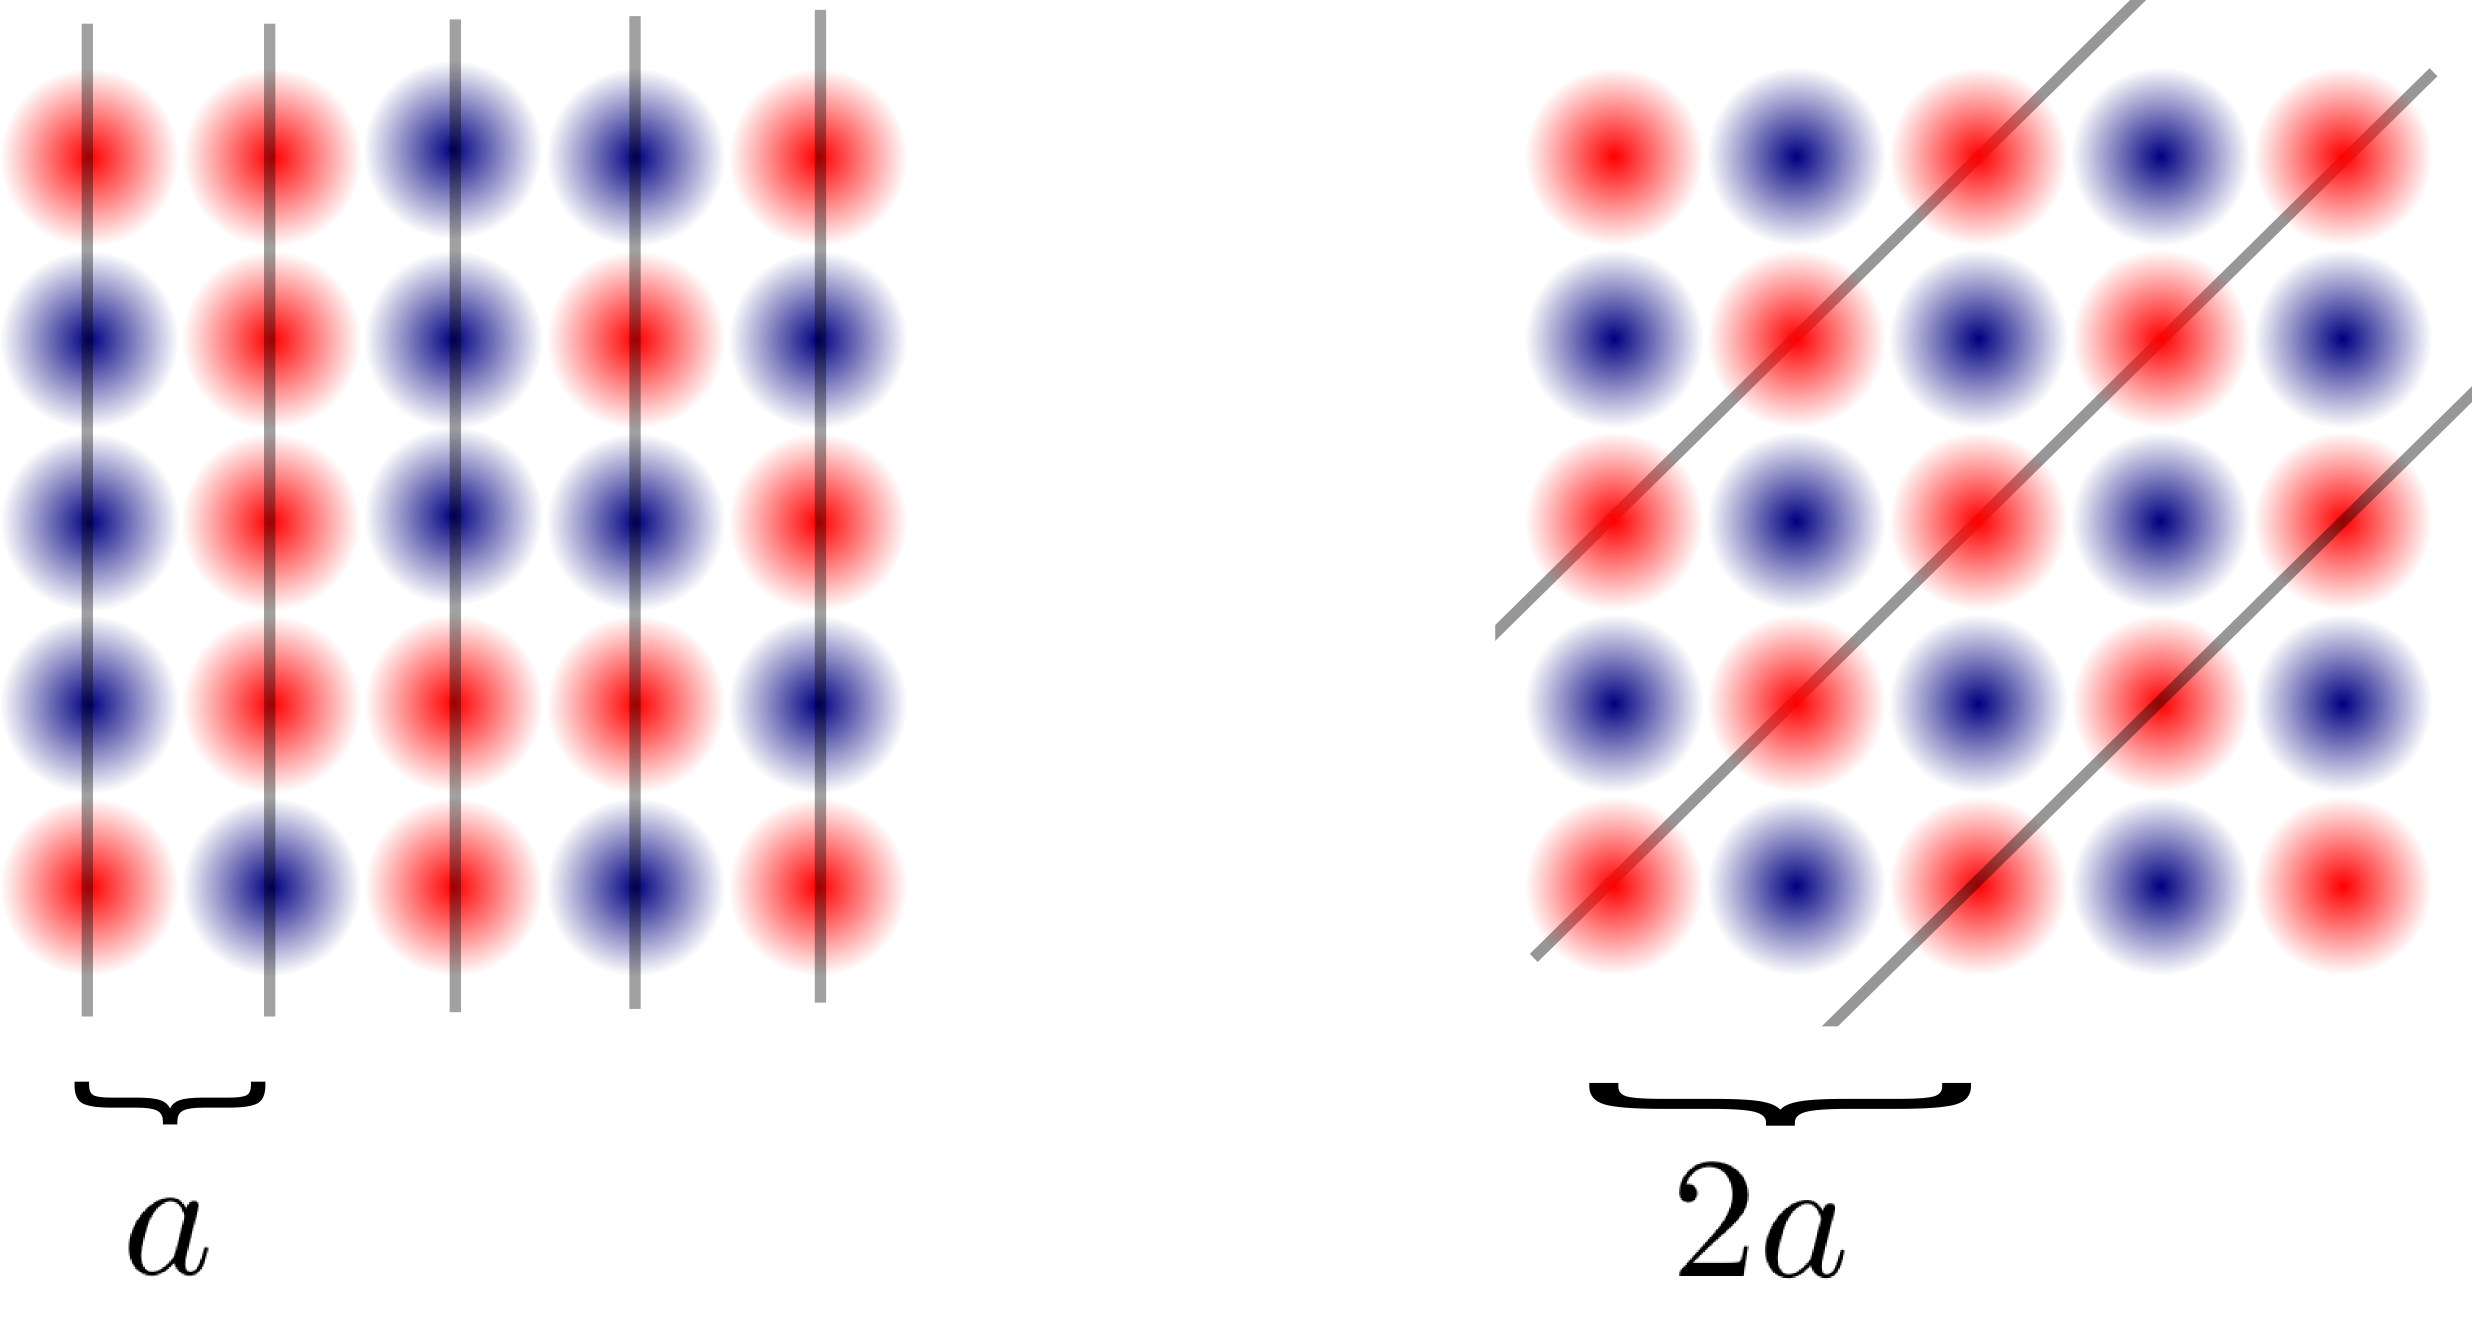
\includegraphics[width=0.5\textwidth]{../figures/braggscatt/magnetic_sublattice_2d.png}
\caption{\small  Illustration of disordered spins in a square optical lattice
(left).  When the spins order antiferromagnetically, a face-centered square
lattice (right) is formed, which has twice the lattice spacing as the
underlying optical lattice. Planes relevant for Bragg scattering are indicate
by the gray lines.  The situation is analogous in three dimensions.  }
\label{fig:magnetic-sublattice}
\end{figure}

In an analogous way to the crystal structure factor we define the spin
structure factor, which is a measure of the spin order of the ensemble, as 
\begin{equation}
 \sq = \frac{1}{N} 
   \sum_{m, n}
  4
  \langle \sigma_{z} \rangle_{m}  \langle \sigma_{z} \rangle_{n}
  e^{ i \bv{Q} \cdot ( \bv{R}_{n} - \bv{R}_{m} ) }   
\label{eq:defineSq}
\end{equation} 
and we can relate it to the measured intensity as 
\begin{equation}
\begin{split}
 I_{\bv{Q}}^{\mathrm{spin}}/A  &   = 
  \debyew 
\frac{  2 s_{0} \Delta^{2}}{ (4\Delta^{2} + s_{0}+1)^{2} }
  N( \sq - 1 ) +   
   N \frac{ s_{0}/2}{ 4\Delta^{2} + s_{0}+1} 
\end{split}
\end{equation}

\subsection{ Time-of-flight} 


We have seen that the Debye-Waller factor,  \debyew\ depends on the spatial
extent of the atomic wavefunctions.   It appears in front of the interference
term for both $I_{\bv{Q}}^{\mathrm{crystal}}$ and $I_{\bv{Q}}^{\mathrm{spin}}$.
If the atoms confined to the locked lattice have a position variance given by
$\langle r_{i}^{2} \rangle_{0}$,  then after releasing them in time-of-flight
(TOF) the variance will evolve according to  
\begin{equation}
\begin{split} 
  \langle r_{i}^{2} \rangle_{\tau} = &
   \langle r_{i}^{2} \rangle_{0} + 
  \frac{\tau^{2}}{m^{2}} \langle p_{i}^{2} \rangle_{0} \\
  = &  \langle r_{i}^{2} \rangle_{0} + 
  \frac{\tau^{2}}{m^{2}} \frac{\hbar^{2}}{4  \langle r_{i}^{2} \rangle_{0} } \\
\end{split}
\end{equation} 
In a harmonic oscillator potential 
\begin{equation}
    \langle r_{i}^{2} \rangle = \frac{\hbar}{2 m \omega_{i}}
\end{equation}
and for a lattice with spacing $a$ and depth $v_{0}$,  
%$\hbar \omega = 2 E_{R}
%\sqrt{V_{0}}$, and 
\begin{equation}
    \langle r_{i}^{2} \rangle = \frac{a^{2}}{ 2 \pi^{2} \sqrt{v_{0}/E_{r}} }
\end{equation}
After some time-of-flight, $\tau$, the Debye-Waller factor will be 
\begin{equation}
\begin{split}
    \debyew =& e^{-2W_{\bv{Q}}(\tau=0) } \exp\left[
-\frac{\sqrt{v_{0}/E_{r}}}{2} \left( \frac{ |\bv{Q}| h }{2 m a  } \right)^{2}
\tau^{2}   \right] \\
\label{eq:bragg-tof-decay}
\end{split}
\end{equation}
For a sufficiently long TOF, which we indicate with the subscript $\infty$, the
Debye-Waller factor goes to zero and the intensity at the detector will consist
only of the non-interfering part:
\begin{equation}
  I_{\bv{Q}\infty}  = A \frac{ N s_{0} / 2}{ 4 \Delta^{2} + s_{0}+1 } 
\end{equation}

Using the above expression for the intensity after long TOF, we can rewrite the
expressions for the crystal and structure factors in the simple form:
\vspace{0.3em}
\begin{equation} 
\boxed{
  \frac{ I_{\bv{Q}}^{\mathrm{crystal}} }{ I_{\bv{Q}\infty}^{\mathrm{crystal}}} =
   C_{\bv{Q}}^{-1}  ( \scrys -1 ) + 1  }
  ~~~~~~~~~~~~\mathbf{crystal\ structure}
\label{eq:crystalstruct}
\end{equation} 
\begin{equation} 
\boxed{
  \frac{ I_{\bv{Q}} }{ I_{\bv{Q}\infty}} = 
   C_{\bv{Q}}^{-1}  ( \sq -1 ) + 1   }
  ~~~~~~~~~~~~~~~~\mathbf{spin\ structure}
\vspace{0.8em}
\label{eq:spinstruct}
\end{equation} 
where we have defined the correction factor $C_{\bv{Q}}$ as 
\begin{equation}
  C_{\bv{Q}} = e^{2W_{\bv{Q}}(\tau=0) }\left( \frac{ 4\Delta^{2} +  s_{0}  +
1}{ 4 \Delta^{2} } \right) \approx e^{2W_{\bv{Q}}(\tau=0) }\left( 1 + \frac{
s_{0} }{ 4 \Delta^{2} } \right),
\label{eq:defineCq}
\end{equation}
where the approximation holds if $4\Delta^{2},s_{0} \gg 1$.  This correction
factor allows us to obtain the crystal and spin structure factors from the
ratio of \textit{in-situ} and TOF measurements of the intensity at $\bv{Q}$.
The correction takes care of accounting for the finite spatial extent of the
wavefunctions in the locked lattice, and also accounts for saturation of the
atomic transition due to the intensity and detuning of the probe light.  
 

\subsection{ Suppression of scattering in other directions}
\label{subsec:suppress}

As can be seen from Eq.~\ref{eq:crystalstruct} and Eq.~\ref{eq:spinstruct}, the
generic form for the scattered intensity is 
\begin{equation}
  \frac{ I_{\bv{Q}} }{ I_{\bv{Q}\infty}} = 
   C_{\bv{Q}}^{-1}  ( S_{\bv{Q}} -1 ) + 1 ,
\end{equation}
where a generic structure factor can be written as
\begin{equation}
 S_{\bv{Q}} = \frac{1}{N} 
  \sum_{m,n} 
  e^{i\bv{Q}\cdot(\bv{R}_{m} - \bv{R}_{n})} f_{c}(\bv{R}_{m}, \bv{R}_{n}),
\end{equation}
where $f_{c}$ is a correlation function.  In most practical cases (e.g. the crystal and magnetic structure discussed above), the correlation function for a fully ordered sample can be written as 
\begin{equation}  
  f_{c}(\bv{R}_{m}, \bv{R}_{n}) = 
  f_{0} e^{i\bv{Q}_{0} \cdot(\bv{R}_{m} - \bv{R}_{n})} ,
\end{equation}
which leads to
\begin{equation}
 S_{\bv{Q}} = \frac{f_{0}}{N} \sum_{m,n}
e^{i(\bv{Q}-\bv{Q}_{0})\cdot(\bv{R}_{m} - \bv{R}_{n})} 
\end{equation}

It is interesting to note that as the size of the sample increases (the sums over $n,m$ extend from $-\infty$ to $+\infty$)  the structure factor approaches a sum of delta functions:
\begin{equation}   
 S_{\bv{Q}} \approx f_{0}  \sum_{m=-\infty}^{\infty}
e^{i(\bv{Q}-\bv{Q}_{0})\cdot \bv{R}_{m}} =  
 f_{0}\left(\frac{2\pi}{a}\right)^{3} \sum_{i,j,k} \delta\left[ \bv{Q}-\bv{Q}_{0} - \frac{2\pi}{a}\ijk \right]
\end{equation}
where $i,j,k$ are integers running from $-\infty$ to $+\infty$.  The collection
of momentum transfers given by $\bv{Q}_{B} = \lbrace \bv{Q}_{0} -
\frac{2\pi}{a}\ijk \rbrace$ corresponds to all of the Bragg peaks exhibited by
the fully ordered system.

If $\bv{Q}_{\text{off}}$ is away from the Bragg condition, $\bv{Q}_{\text{off}}
\notin \bv{Q}_{B}$, we have $ S_{\bv{Q}_{\text{off}}} = 0 $ and 
\begin{equation}
  \frac{ I_{\bv{Q}} }{ I_{\bv{Q}\infty}} = 
  1 - C_{\bv{Q}}^{-1} 
\end{equation}

It can be seen that the presence of the fully ordered sample suppresses
scattering of light in directions that do not satisfy the Bragg condition.  If
the scattering conditions are fully coherent $C_{\bv{Q}} = 1 $ and the
suppression of light scattered away from the Bragg peaks is total.  


\section{Experimental setup} 

One of the limitations when doing Bragg scattering in an ultracold atom
experiment is the lack of sufficient optical access to setup the vectors
$\bv{k}$ and $\bv{k}'$ of the input and output light such that the momentum
transfer, $\bv{Q}$, matches a vector or the reciprocal crystal lattice or the
reciprocal magnetic sublattice.  The orientation of the lattice in the vacuum
chamber, the lattice spacing, and the wavelength of the light define the
possible angles at which the Bragg condition will be satisfied. 

We have implemented setups to guarantee access to two values of the momentum
transfer. One of them corresponds to scattering from the \zoz\ lattice planes,
and the other one corresponds to scattering from the \hhh\ magnetic sublattice
planes.   Both cases are illustrated in
Fig.~\ref{fig:bragg_crystal_spin_angles}.
\begin{figure}
    \centering
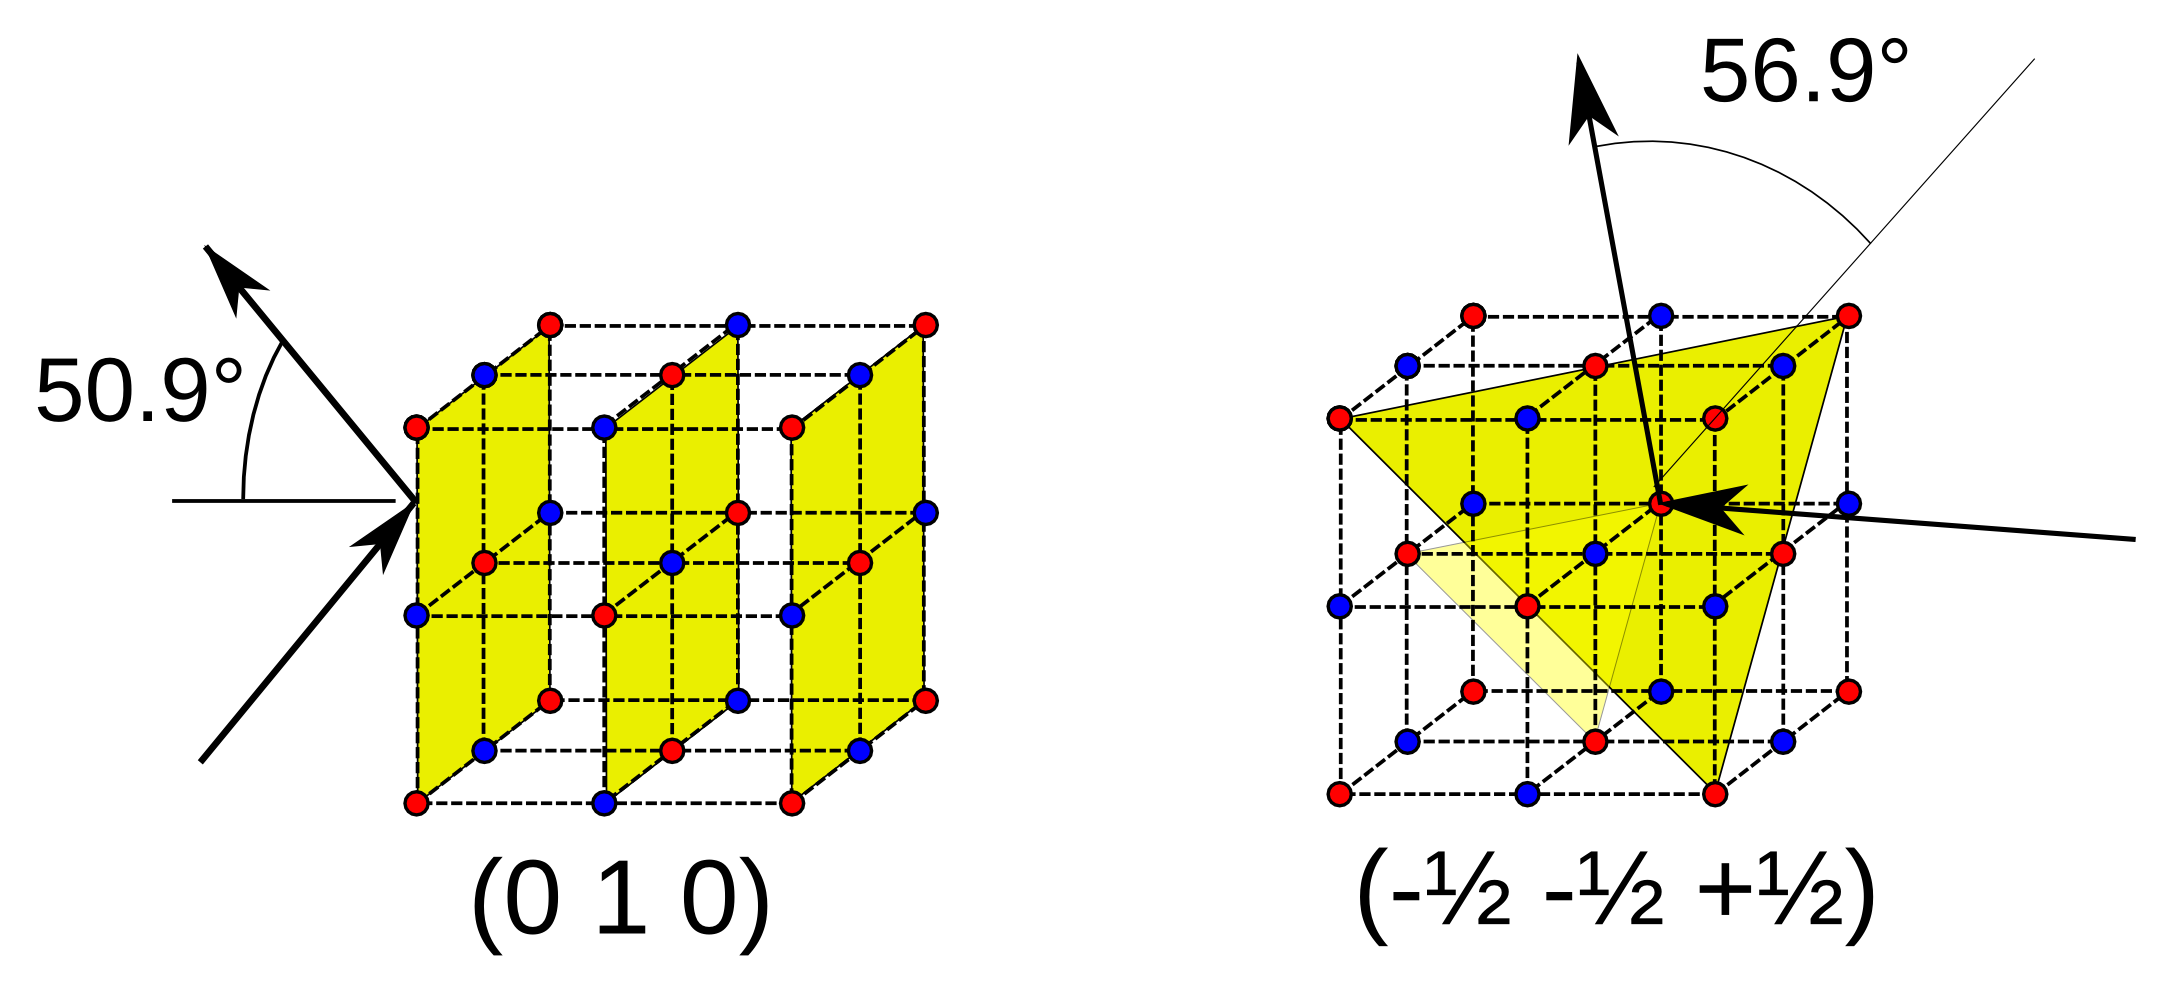
\includegraphics[width=0.75\textwidth]{../figures/braggscatt/bragg_crystal_spin_angles.png}
\caption{\small  Illustration of the angles involved in Bragg scattering.  The
crystal structure factor is addressed by scattering off of the \zoz\ lattice
planes, and the spin structure factor is addressed by scattering off of the
\hhh\ magnetic sublattice planes. }
\label{fig:bragg_crystal_spin_angles}
\end{figure}
The situation for the \hhh\ scattering with respect to our vacuum chamber is
shown in Fig.~\ref{fig:bragg_hhh_chamber}.   In the figure, the lattice beams
propagate along $x$, $y$ and $z$.  To facilitate the alignment of the \hhh\
input beam we planned for it to lie on the $yz$-plane.  To satisfy the Bragg
condition, the direction of propagation of the Bragg input beam makes an angle
of $3.06^{\circ}$ with the positive $y$-axis.  The input beam for the \zoz\
scattering direction (not shown in the Fig.~\ref{fig:bragg_hhh_chamber}) is
also selected to lie on the $yz$-plane.  It propagates along a line that makes
an angle of $50.9^{\circ}$ with the negative $y$-axis. 
\begin{figure}
    \centering
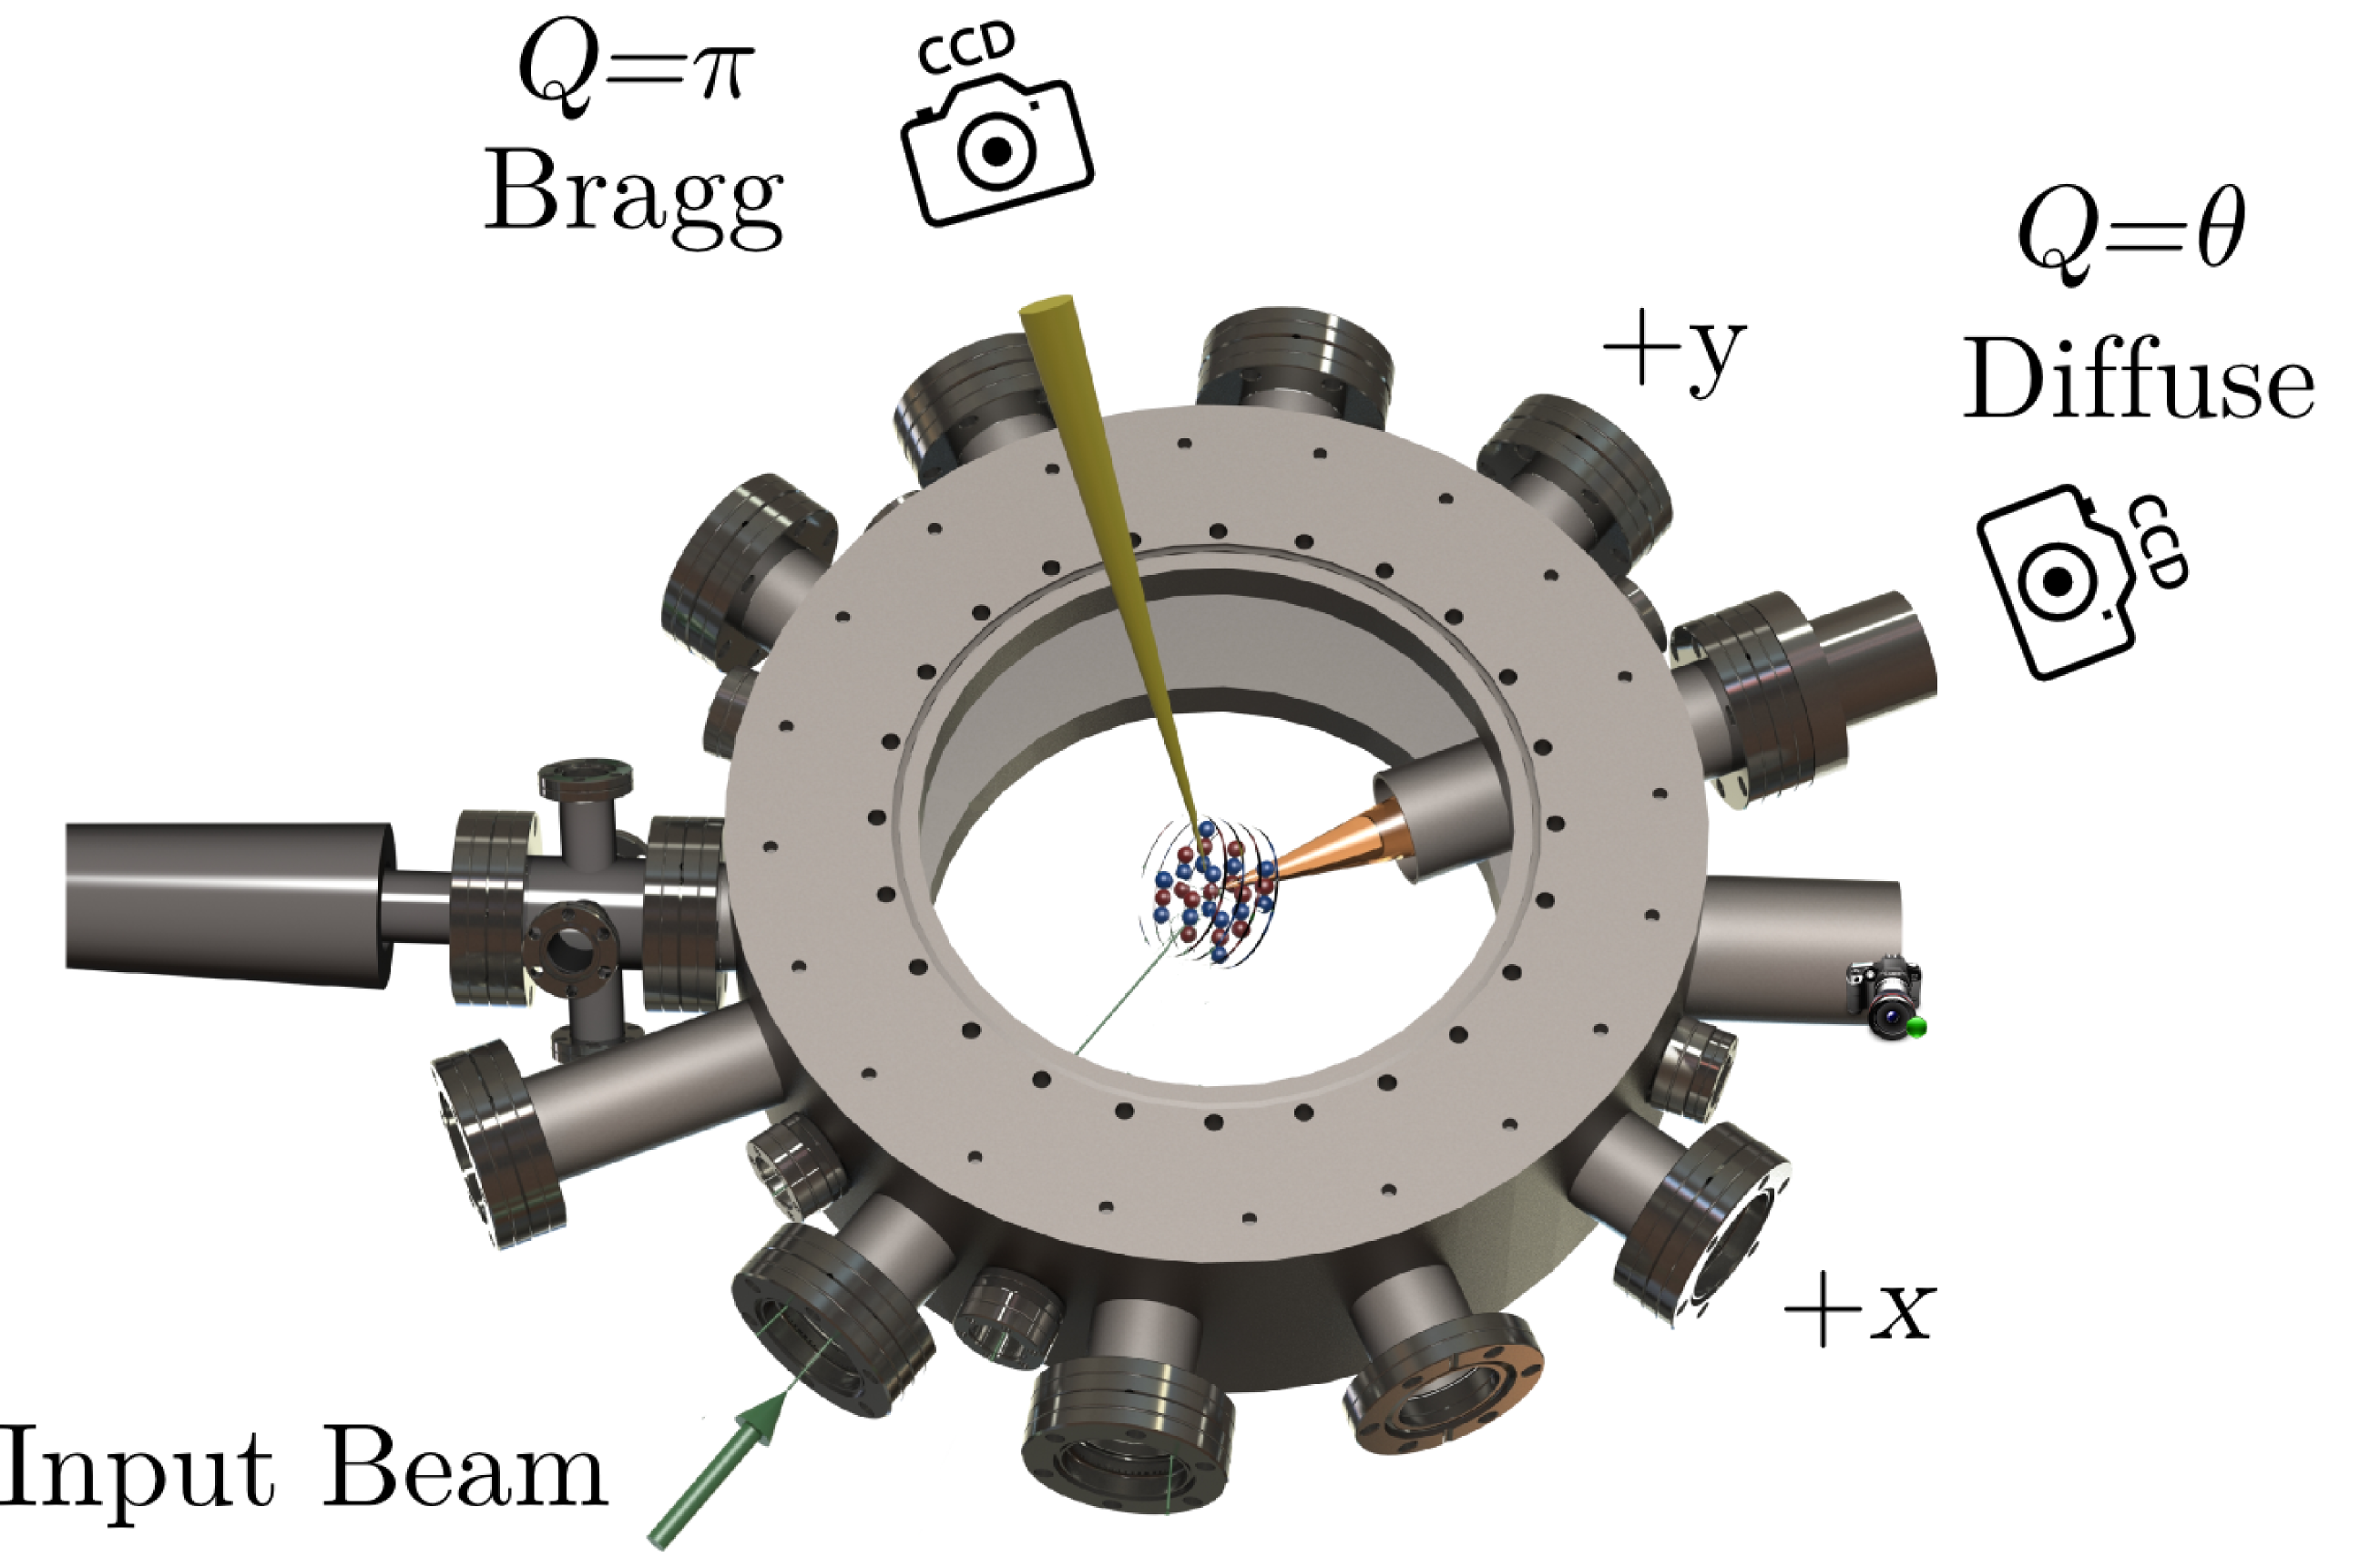
\includegraphics[width=0.7\textwidth]{../figures/braggscatt/bragg_hhh_setup_chamber.png}
\caption{\small  Experimental setup for the \hhh\ Bragg scattering direction,
showing the vacuum chamber.  The momentum transfer $\bv{Q}$ for Bragg scattering
off of the \hhh\ magnetic sublattice is denoted as $\bv{\pi}$.  An additional
imaging viewport allows us to measure the light scattered in a direction that
does not satisfied the Bragg condition, labeled as $\bv{Q}=\bv{\theta}$. }
\label{fig:bragg_hhh_chamber}
\end{figure}

The illustration in Fig.~\ref{fig:bragg_hhh_chamber} has the top viewport of
the vacuum system removed.  The reader may remember that we have a re-entrant
viewport on the top, and that the magnetic coils sit inside the re-entrant
viewport to be close to the atoms (refer to Fig.~\ref{fig:coilforms}).  In
Fig.~\ref{fig:bragg-outputs} we show the optical setup used to guide the output
Bragg light from the atoms to an imaging system and CCD camera, where the light
is collected.    
\begin{figure}
    \centering
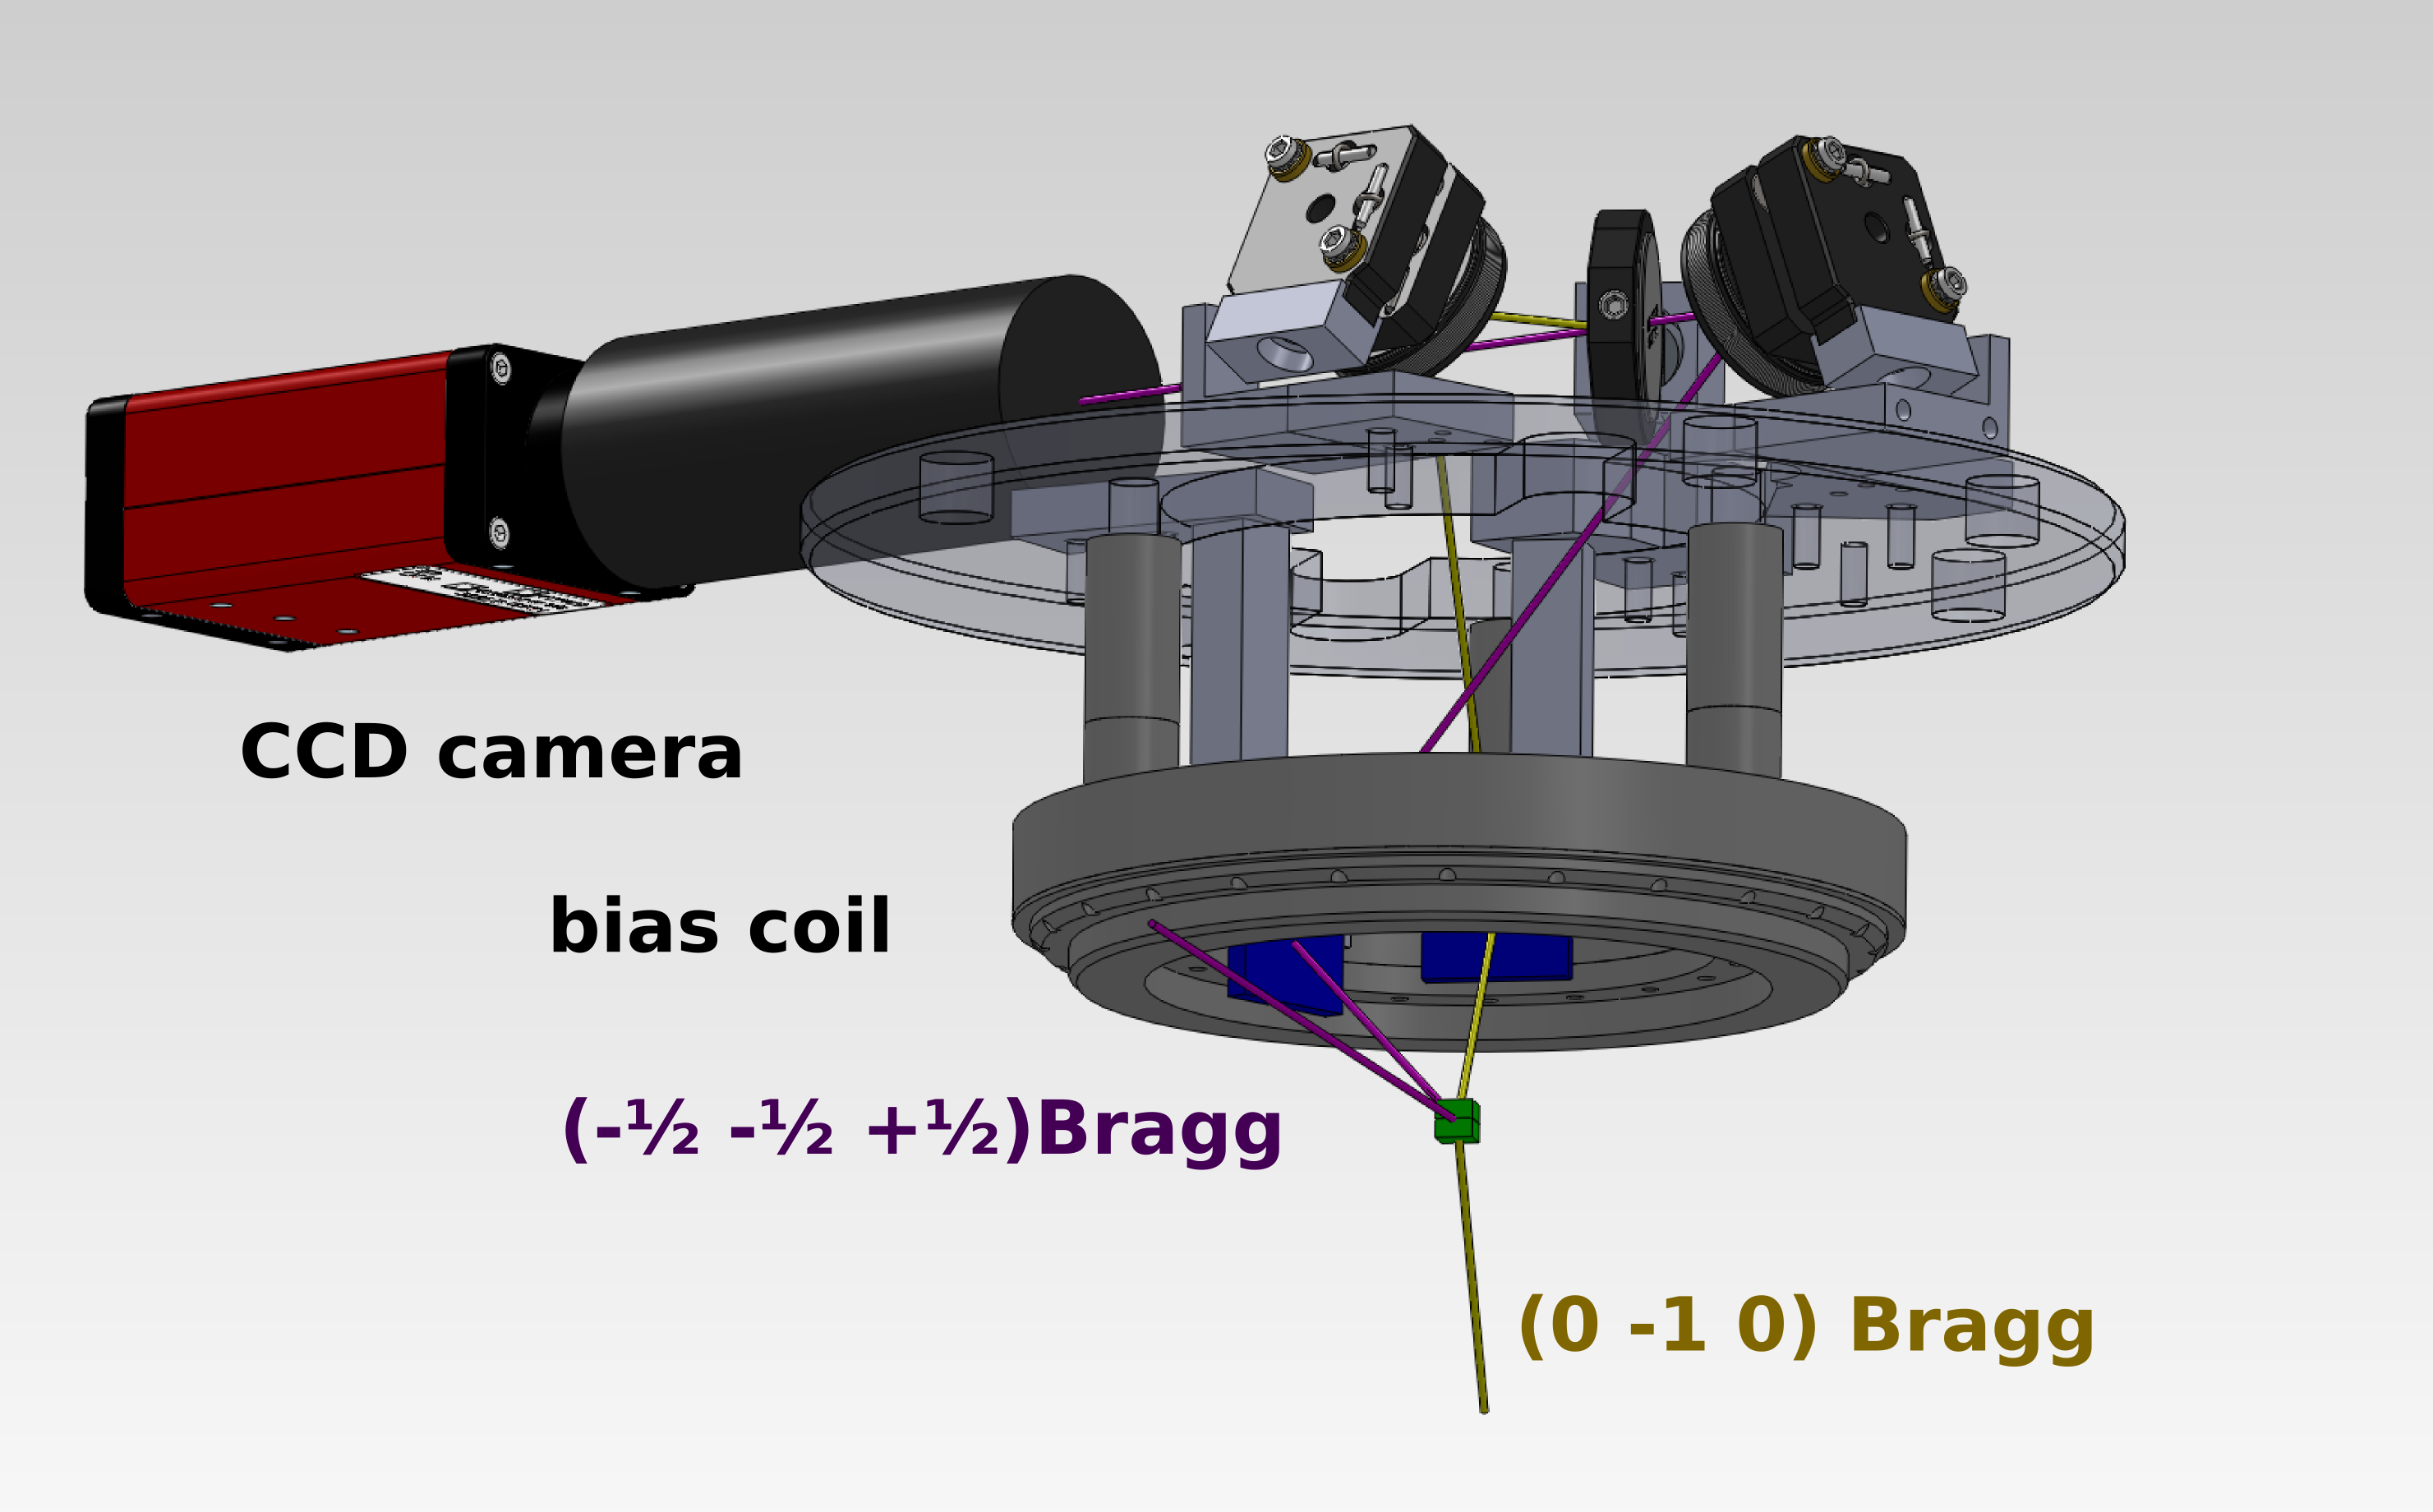
\includegraphics[width=0.7\textwidth]{../figures/braggscatt/bragg_initial_setup_updated.png}
\caption{\small  Optical setup to guide the output Bragg light to the CCD for
detection.  Two drop-down mirrors are positioned inside the re-entrant viewport
to reflect the Bragg output light for the \zoz\ and \hhh\ setups. In both cases
the light is reflected by a second mirror positioned on the rim of the
re-entrant viewport.  A removable mirror allows to select whether the \zoz\ or
the \hhh\ output light goes to the imaging setup.  }
\label{fig:bragg-outputs}
\end{figure}

\subsection{Diffuse background} 

In addition to the CCD camera used for dedicated imaging of either the crystal
or spin structure factor,  we have at our disposal the camera that is regularly
used to image the atom cloud.    Keeping the same direction of the Bragg input
beam, and measuring the scattered light at a direction that does not satisfy
the Bragg condition provides an alternative background for the Bragg scattering
measurement, in addition to the normalization done with an uncorrelated sample
after long TOF. Figure~\ref{fig:bragg_hhh_chamber} illustrates this additional
imaging direction, which we refer to as ``diffuse''.


\section{ Measurement of the crystal structure factor} 

As a test of our ability to do Bragg scattering, and also to find out the
practical limits of sensitivity for this technique, we set out to measure the
crystal structure factor along the \zoz\ scattering direction.  We used a
sample in an uncompensated lattice, for the simple reason that we do not have
to guarantee the proper alignment of the compensation beams to perform the
experiment.  We also used a surveillance CCD camera, which does not have the
best noise characteristics.   As we will explain later on, when we went on to
measure Bragg scattering in the \hhh\ direction we had to make use of a low
noise cooled CCD camera. 

Figure~\ref{fig:100dwfactor} shows a measurement of the Bragg
scattered light versus the lock depth of the lattice.  For larger lock depth,
$v_{0}$, the Debye-Waller factor increases as 
\begin{equation}
   e^{-2W_{\bv{Q}}(\tau=0)}   = \exp\left[
-\frac{a^{2}|\bv{Q}|^{2}}{2\pi^{2}\sqrt{v_{0}/E_{r}}} \right] = \exp\left[ -
\frac{2}{\sqrt{v_{0}/E_{r}}} \right], 
\end{equation}
where the last expression holds for $\bv{Q}=\bv{\theta} = \frac{2\pi}{a}\zoz$.
\begin{figure}
    \centering
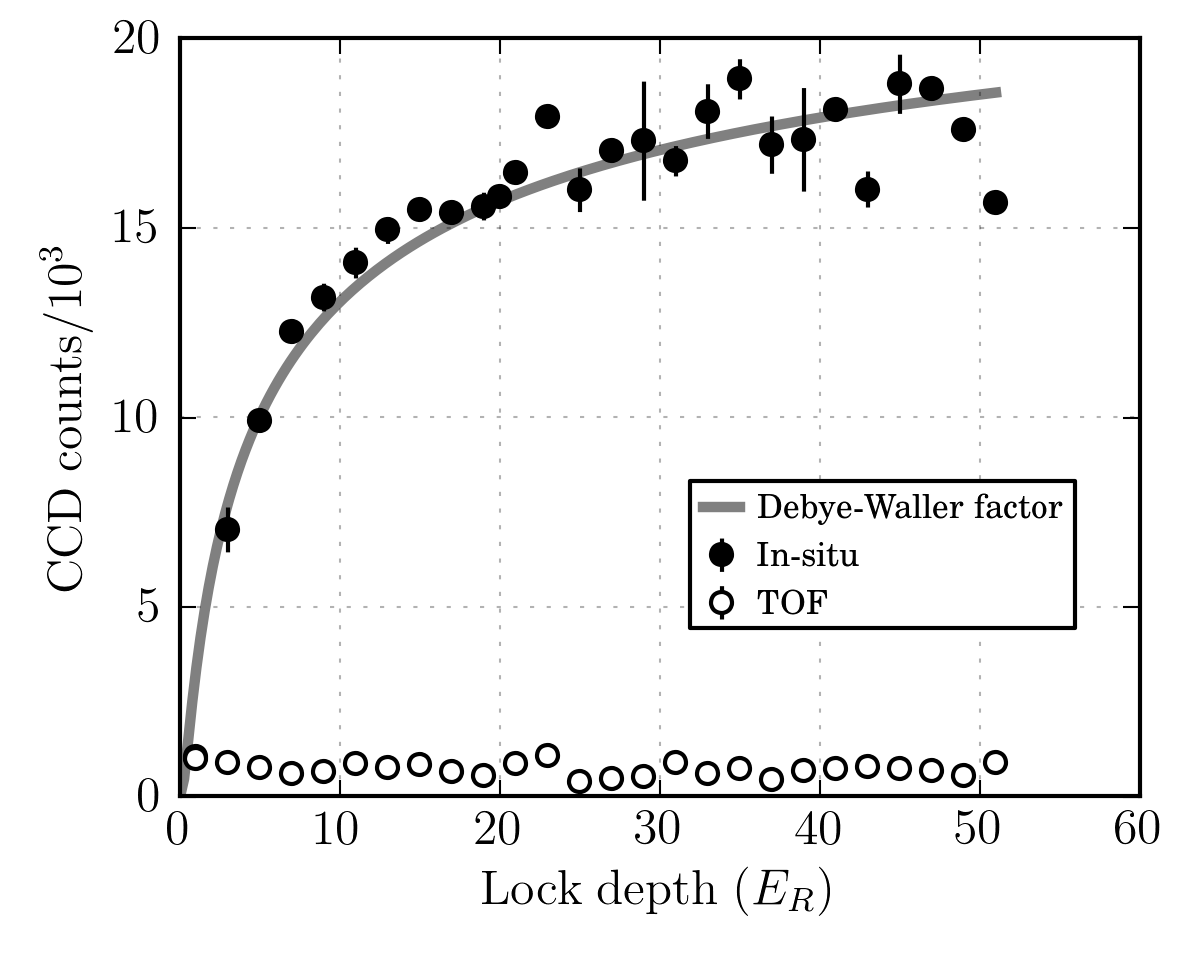
\includegraphics[width=0.6\textwidth]{../figures/braggscatt/dwfactorNice2.png}
\caption{\small  Measurement of Bragg scattering signal vs. lock depth.  The
Bragg probe used had a waist of 500~$\mu$m and a 200\,$\mu$W of power, for a
saturation parameter $s_{0}=10.0$.   The detuning used was $-28$~MHz
($-4.7\Gamma$) from state $|2\rangle$, which is -104~MHz (-17.6$\Gamma$ ) from
state $|1\rangle$.  The exposure time was 1.7~$\mu$s. A measurement taken after
a long TOF (6~$\mu$s) shows the uncorrelated scattering background.   }
\label{fig:100dwfactor}
\end{figure}

Releasing the atoms in time of flight reveals the expansion of the atomic
wavefunction, causing a decay of the Bragg scattering signal in a very short
time of only a few micro seconds, as shown in Fig.~\ref{fig:100tof}. 
\begin{figure}
    \centering
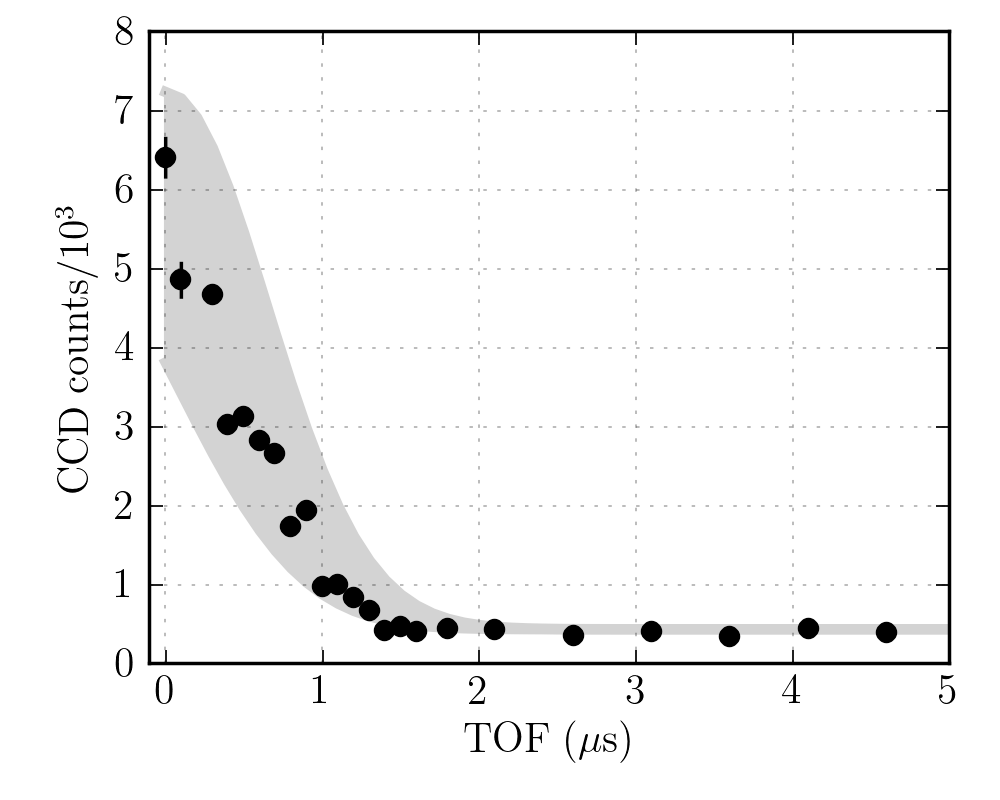
\includegraphics[width=0.6\textwidth]{../figures/braggscatt/tofNice2.png}
\caption{\small  Measurement of Bragg scattering signal vs. TOF.  The lattice
depth was locked to 20\,$E_{r}$.  For this measurement the power, waist and
exposure of the probe are the same as in Fig.~\ref{fig:100dwfactor}.  The
detuning is $-53$~MHz ($-9.0\Gamma$) from state $|2\rangle$ which is -129~MHz
(-21.9$\Gamma$ ) from state $|1\rangle$, resulting in a lower overall signal
than is seen in Fig.~\ref{fig:100dwfactor} at a lock depth of 20\,$E_{r}$.  The
top of the shaded region is calculated using the expression in
Eq.~\ref{eq:bragg-tof-decay}, and the bottom is calculated using the average of
the Eq.~\ref{eq:bragg-tof-decay} during the 1.7\,$\mu$s duration of the probe
exposure.  }
\label{fig:100tof}
\end{figure}


\subsection{Angular dependence of the scattering} 

We also measured the variation of the Bragg scattering signal with respect to
the angle of the input beam.  For this measurement we kept the \zoz\ input
Bragg beam in the $yz$-plane and varied the angle it makes with the $xz$-plane.
The results are shown in Fig.~\ref{fig:100rocking}. 
\begin{figure}
    \centering
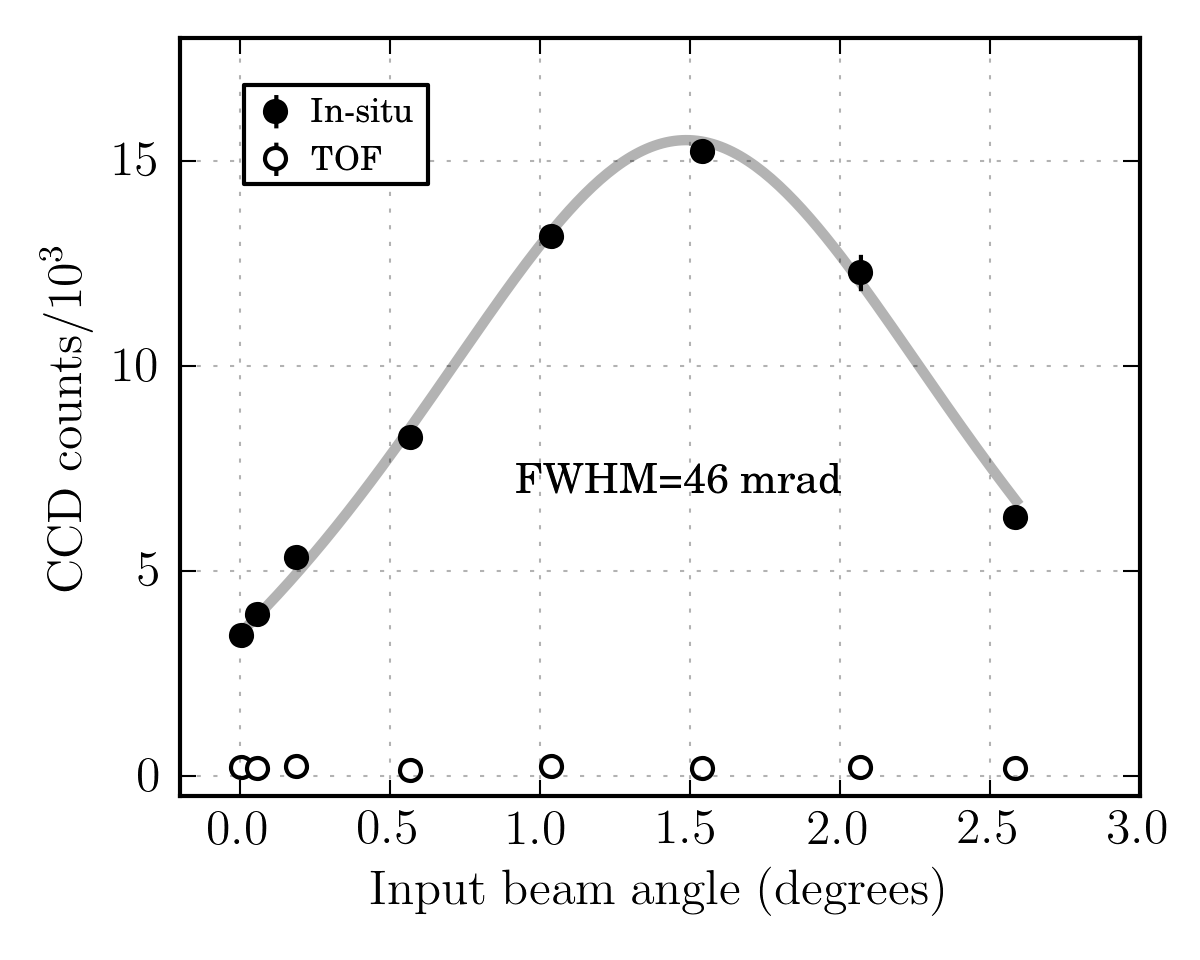
\includegraphics[width=0.6\textwidth]{../figures/braggscatt/rockingNice3.png}
\caption{\small  Measurement of Bragg scattering signal vs. input angle of the
Bragg probe. The label shows the $1/e$ radius of the Gaussian
fit, determined to be 21~mrad.  }
\label{fig:100rocking}
\end{figure}
From a measurement of the full width at half-max (FWHM) of the angular
distribution one can obtain the correlation length of the sample.   In this
case every atom is localized at a lattice site, and all of the them contribute
constructively to the Bragg scattered signal in the detector (up to the extent
of their wavefunction, given by the Debye-Waller factor).  The correlation
length must then be indicative of the size of the entire sample.   

In order to relate the width of the angular distribution to the correlation
length, one must assume some functional form for a correlation function.  Since
we are working on a lattice, a generic structure factor can be calculated as
the following sum over lattice sites (see Chapter 2 in
\cite{chaikin2000principles})
\begin{equation}
  F_{\bv{Q}} =  \frac{1}{N} \sum_{i,j} 
  e^{i\bv{Q} \cdot (\bv{R}_{i} - \bv{R}_{j}) }
    f_{c}(\bv{R}_{i},\bv{R}_{j} )
%    f_{c}(|\bv{R}_{m}-\bv{R}_{n}| )
\end{equation}
where $f_{c}(\bv{R}_{i},\bv{R}_{j} )$ is the correlation function.  For the
crystal structure factor we have  
\begin{equation}
 f_{\text{Crystal}}(\bv{R}_{i},\bv{R}_{j} ) =   \langle n_{i} n_{j} \rangle 
\end{equation}
where $n_{i}$ is the density operator at the $i^{\text{th}}$ site.  And for the
magnetic structure factor  
\begin{equation}
 f_{\text{Spin}}(\bv{R}_{i},\bv{R}_{j}) =  
     4 \langle \sigma_{zi} \sigma_{zj} \rangle 
\end{equation}
where $\sigma_{zi}$ is the $z$-component of the spin operator at the
$i^{\text{th}}$ site.



%For a completely correlated sample with a finite extent, this function may be
%a box function given by \begin{equation} f_{c}( |\bv{R}_{m}-\bv{R}_{n}| ) =
%\begin{cases}  1 &   \text{if}\ |\bv{R}_{m}-\bv{R}_{n}| \leq L_{\text{AFM}}\\
%0           &   \text{if}\ |\bv{R}_{m}-\bv{R}_{n}| > L_{\text{AFM}}\\
%\end{cases} \end{equation}


As an example, if correlations are starting to form on the approach to a
magnetic phase transition the spin correlation function may be taken to be
equal to the density correlation function multiplied by an exponential: 
\begin{equation}
 f_{\text{Spin}}( \bv{R}_{i},\bv{R}_{j} ) =  \langle n_{i} n_{j} \rangle
  e^{i\bv{\pi} \cdot (\bv{R}_{i} - \bv{R}_{j}) }     
     e^{-|\bv{R}_{i} - \bv{R}_{j}| / L_{c} } 
\label{eq:spin-corr-fun}
\end{equation}
%These two functions are plotted in Fig.~\ref{fig:corr-fun}. 
%\begin{figure}
%    \centering
%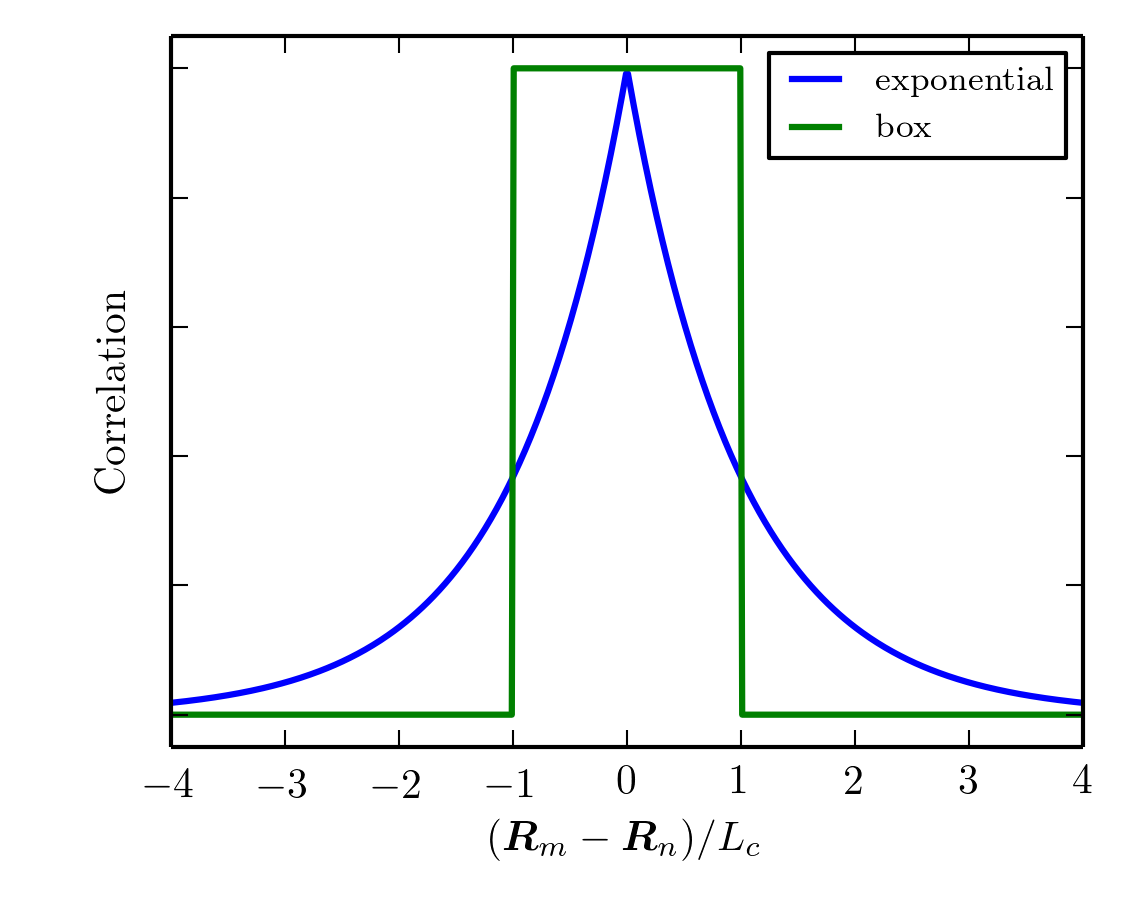
\includegraphics[width=0.5\textwidth]{../figures/braggscatt/correlation-fun.png}
%\caption{\small  Box and exponential correlation functions.  }
%\label{fig:corr-fun}
%\end{figure}

%In terms of the correlation function, a generic structure factor can be written
%as 
%\begin{equation}
%  F_{\bv{Q}} =  \frac{1}{N} \sum_{m,n} e^{i\bv{Q} \cdot (\bv{R}_{m} - \bv{R}_{n}) }
%    f_{c}(|\bv{R}_{m}-\bv{R}_{n}| )
%\end{equation}

We wish to obtain the angular dependence of the structure factor in the
vicinity of $\bv{Q}_{0}$,  where the Bragg condition is fulfilled at
$\bv{Q}=\bv{Q}_{0}$ (which in the case of crystal order implies
$e^{i\bv{Q}_{0}(\bv{R}_{m}-\bv{R}_{n})}=1$ for all $m,n$).  We define the small
vector $\bv{p} = \bv{Q}-\bv{Q}_{0}$.  In terms of $\bv{p}$ a generic structure
factor can be written as
%and splitting the sum into $m=n$ and $m\neq n$ parts:
\begin{equation}
\begin{split} 
F(\bv{p})  & = 
   \frac{1}{N}
   \sum_{i,j}
%\left(  
%   \sum_{i} + 
%      \sumOffij \right) 
      e^{ i \bv{p}( \bv{R}_{i} - \bv{R}_{j} ) } 
   f_{c}( \bv{R}_{i},\bv{R}_{j} )  \\ 
%%   & \approx 
%%  1+ 
%%      \sum_{k}  
%%      e^{ i \bv{p}\bv{R}_{k} } 
%%   f_{c}(  |\bv{R}_{k}| )  
%   e^{-|\bv{R}_{k}| / L_{c} }  
\end{split}
\end{equation}

We will assume that the expectation value factorizes as $\langle n_{i} n_{j}
\rangle = \langle n_{i} \rangle \langle n_{j} \rangle $.   If we assume that
the density distribution of the atoms is Gaussian we have 
\begin{equation}
  \langle n_{i} \rangle =  n_{0} e^{ - R_{i}^{2}/\sigma^{2}}
\end{equation} 
and 
\begin{equation}
\begin{split} 
F(\bv{p})  & = 
   \frac{1}{N}
   \sum_{i} 
      e^{ i \bv{p} \cdot \bv{R}_{i}}  n_{0} e^{ - R_{i}^{2}/\sigma^{2}}
   \sum_{j} 
      e^{ -j \bv{p} \cdot \bv{R}_{j} } n_{0} e^{ - R_{j}^{2}/\sigma^{2}} \\ 
   & =\frac{1}{N}
   \left| \sum_{i} 
      e^{ i \bv{p} \cdot \bv{R}_{i}}  n_{0} e^{ - R_{i}^{2}/\sigma^{2}} \right|^{2}
\end{split}
\end{equation}
The sum can be approximated as an integral to obtain 
\begin{equation}
F(\bv{p})   \approx 
  \frac{1}{N} 
  \left[ 
   \frac{n_{0}}{ a^{3}} 
   \int_{\mathbb{R}^{3}} \mathrm{d}\bv{R}_{i}  \,
      e^{ i \bv{p}\bv{R}_{i}  }  
    e^{ - R_{i}^{2}/\sigma^{2}} \right]^{2}
\end{equation} 
The Fourier transform of a spherically
symmetric function in three dimensions is equivalent to the Fourier-Bessel
transform of the radial function, so we have: 
\begin{equation}
F(\bv{p})   \approx
  \frac{1}{N} \left[ 
   \frac{n_{0}}{ a^{3}} 4 \pi  
   \int_{0}^{\infty} 
    e^{ - R^{2}/\sigma^{2}}
   \frac{ \sin(pR)}{pR}\, R^{2} 
   \mathrm{d}R  \, \right]^{2}
\end{equation}
This integral can be carried out analytically to obtain
\begin{equation}
\begin{split} 
F(\bv{p}) &  \approx \frac{1}{N}
  \left[   \frac{n_{0}}{ a^{3}} 4 \pi 
  \frac{ \sqrt{\pi} \sigma^{3} }{4} e^{-p^{2} \sigma^{2} / 4 }  \right]^{2} \\
& \propto e^{-p^{2} \sigma^{2} / 2 }
\end{split}
\end{equation}
If one changes the angle of the input vector by a small amount $\delta\alpha$
(measured in radians)  then, to first order, the magnitude of $\bv{p}$ changes
as $\delta p = \frac{2\pi}{\lambda_{0}} \delta\alpha$, where $\lambda_{0}$ is
the wavelength of the Bragg probe. The final result for the angular
distribution of the scattered light is then
\begin{equation}
F(\delta\alpha)   \propto
  \exp\left[  - \frac{ 2  (\delta\alpha)^{2} }
       { \lambda_{0}^{2} / (\sigma^{2} \pi^{2}) } \right]   
\end{equation}
which has a FWHM given by $ \frac{2 \sqrt{2\ln2}}{2 \pi}
\frac{\lambda_{0}}{\sigma} \approx 0.37 \lambda_{0} / \sigma $. 

The measurement shown in Fig.~\ref{fig:100rocking}, which has a FWHM$=46\,$mrad
would then be consistent with a cloud with $1/e$ radius  $\sigma = 5\,\mu$m.
The $1/e$ radius of the cloud in the uncompensated lattice is measured to be
$\sim10~\mu$m.   According to the analysis presented, the measured angular
distribution should have been narrower by a factor of 2.   This is somewhat
disconcerting because one would expect those two results to agree.   The
discrepancy may point at an issue with our calibration of the angular
displacement of the probe beam as it was varied in our setup.


In the case of a measurement of the magnetic structure factor in a sample that
has developed AFM spin correlations one can start with
Eq.~\ref{eq:spin-corr-fun} and perform the Fourier transform, as presented
here, to find out the angular dependence of the scattering signal. 


%\newpage
%%%%%%%%%%%%%%%%%%%%
%
%
%\begin{equation}
%\begin{split} 
%F(\bv{p})  & = 
%   \frac{1}{N}
%   \sum_{i,n}
%%\left(  
%%   \sum_{i} + 
%%      \sumOffij \right) 
%      e^{ i \bv{p}( \bv{R}_{i} - \bv{R}_{j} ) } 
%   f_{c}( \bv{R}_{i},\bv{R}_{j} )  \\ 
%   & \approx 
%  1+ 
%      \sum_{k}  
%      e^{ i \bv{p}\bv{R}_{k} } 
%   f_{c}(  |\bv{R}_{k}| )  
%%   e^{-|\bv{R}_{k}| / L_{c} }  
%\end{split}
%\end{equation}
%where in the last line we have changed variables according to $\bv{R}_{m} =
%\bv{R}_{n} + \bv{R}_{k}$,  and neglected edge effects.  The sum in the last
%term can be approximated as an integral as 
%\begin{equation}
%F(\bv{p}) \approx  
%     1 + 
%   \frac{1}{a^{3}} 
%   \int_{\mathbb{R}^{3}} \mathrm{d}\bv{R}_{k}  \, 
%      e^{ i \bv{p}\bv{R}_{k}  }  
%   f_{c}(  |\bv{R}_{k}| )  
%%   e^{-|\bv{R}_{k}| / L_{c} }  
%   f_{c}(  |\bv{R}_{k}| )  
%\end{equation}
%where $a$ is the lattice spacing.  The Fourier transform of a spherically
%symmetric function in three dimensions is equivalent to the Fourier-Bessel
%transform of the radial function, so we have: 
%\begin{equation}
%\begin{split}
% F(\bv{p})   
%   & \approx 1 +  
%   4 \pi \int_{0}^{\infty} f(R)
%   \frac{ \sin(pR)}{pR}\, R^{2} 
%  \mathrm{d}R
%\end{split}
%\end{equation}
%which can be integrated analytically to obtain 
%\begin{equation}
%F(\bv{p}) \approx 1 +  
%    \frac{8\pi}{a^{3}} 	\frac{ L_{c}^{3} }
%     { \left[ 1 + (L_{c} |\bv{p}|)^{2}  \right]^{2} } 
%\end{equation}
%If one changes the angle of the input vector by a small amount $\delta\alpha$
%(measured in radians)  then, to first order, the magnitude of $\bv{p}$ changes
%as $\delta p = \frac{2\pi}{\lambda_{0}} \delta\alpha$, where $\lambda_{0}$ is
%the wavelength of the Bragg probe. 
%
%The final result for the angular distribution of the scattered light is 
%\begin{equation} 
%\frac{F(\delta\alpha) - 1}{ F(0) } \approx \frac{ 1 } { \left[ 1 +
%\left(\frac{2\pi L_{c}}{\lambda_{B}} \delta\alpha \right)^{2}  \right]^{2} }
%\approx \exp\left[ -2 \left( \frac{2\pi}{\lambda_{B}} L_{c}
%\delta\alpha\right)^{2} \right]
%\end{equation}
%and the $1/e$ radius of the angular distribution is given by 
%\begin{equation}
% \delta\alpha_{1/e} \approx \frac{ \lambda_{B}}{ 2\pi\sqrt{2}} \frac{1}{L_{c}}  
%  =  \frac{ \lambda_{B}/a}{ 2\pi\sqrt{2}} \frac{1}{L_{c}/a}  
%  =   \frac{0.14}{L_{c}/a} 
%\end{equation}
%
%For the \zoz\ Bragg scattering results shown in Fig.~\ref{fig:100rocking},  if
%one assumes an exponential correlation function, the correlation length
%would be $L_{c} = 7a$.  The $1/e$ radius of the cloud in the uncompensated
%lattice is measured to be $13~\mu$m (24$a$).   According to the analysis
%presented, the measured angular distribution should have been narrower.  
%The discrepancy is, most likely, due to the fact that the correlation function
%in the crystal structure case is not exponential, but rather has a sharp cutoff
%at some radius.   Nevertheless, the disagreement points at a possible error on
%the measurement, or maybe hints at the fact the the assumption of a certain
%correlation function can systematically affect an estimate of the correlation
%length obtained from the width of the angular distribution.  
 
\vspace{3em} 

\paragraph{Summary} 

To summarize,  in this chapter we have derived a way to relate measured
intensities to structure factors using Bragg scattering.  The measurement
relies on the ability to realize an uncorrelated sample by simply releasing the
atoms in time of flight.  Corrections due to the finite extent of the atomic
wavefunctions in the lattice (Debye-Waller factor) and due to the saturation of
the atomic transition have been derived.   Taking into account saturation
effects is not necessary for the \zoz\ Bragg scattering, because the light can
be far detuned, but it will be required for spin sensitive Bragg scattering on
the \hhh\ direction, where the detuning is constrained by the spacing between
levels $|1\rangle$ and $|2\rangle$. 

In Chapter~\ref{chap:afmbragg} we will show the results for a measurement of
the spin structure factor, $S_{\bv{Q}}$, in a sample which has developed short
range correlations on the approach to the N\'{e}el transition.  There we will
see that the measurement of $S_{\bv{Q}}$, can be compared to theoretical
calculations in order to establish precise thermometry of the atoms in the
lattice. 

 



